\documentclass[aspectratio=169]{beamer}

% get rid of clickable beamer buttons
\beamertemplatenavigationsymbolsempty

% parse most utf-8 correctly
\usepackage[utf8]{inputenc}
\usepackage[ngerman]{babel}

% better graphics
\usepackage{graphicx}

\title{
    Eine Email-Client-App entwickeln\\
    \vspace{.1cm}
    \normalsize snailmail
}
\author{Noah Vogt \& Simon Hammer}
\date{5. Februar 2022}
\institute{Gymnasium Kirschgarten}

\usetheme{Copenhagen}

\usepackage{varwidth}

\usepackage{graphicx,calc}
\newlength\myheight
\newlength\mydepth
\settototalheight\myheight{Xygp}
\settodepth\mydepth{Xygp}
\setlength\fboxsep{0pt}

\newcommand*\inlinegraphics[1]{
    \settototalheight\myheight{Xygp}
    \settodepth\mydepth{Xygp}
    \raisebox{-\mydepth}{\includegraphics[height=\myheight]{#1}}%
}

% for code snippits
\usepackage{listings}
\usepackage{color}

\definecolor{dkgreen}{rgb}{0,0.6,0}
\definecolor{gray}{rgb}{0.5,0.5,0.5}
\definecolor{mauve}{rgb}{0.58,0,0.82}
\definecolor{background}{rgb}{0.36,0.36,0.36}

\lstset{
    numbersep=3pt,
    keywordstyle=\color{blue},
    commentstyle=\color{dkgreen},
    stringstyle=\color{mauve},
    breaklines=true,
    numbers=left,
    numberstyle=\scriptsize\color{black},
    frame=none,
    basicstyle = \small\ttfamily,
    breaklines=true
    breakatwhitespace=false,
    columns=flexible,
    xleftmargin=0.5cm,framesep=8pt,framerule=0pt,
    aboveskip=3mm,
    belowskip=3mm,
}

% Package to use videos
\usepackage{movie15}
\usepackage{media9}

%for table
\usepackage{array}
\newcolumntype{C}[1]{>{\centering\arraybackslash}m{#1}}

%% Putting the background image in the frames
\usebackgroundtemplate{%
    %\vbox to \paperheight{\hfil\hbox to \paperwidth{\hfil\includegraphics[width=1\paperwidth]{../../logo/version2grey.pdf}\hfil}\vfil}
    \hspace{5.2cm}\includegraphics[width=0.8\paperwidth]{../logo/version2grey.pdf}
    }

\begin{document}
\begin{frame}[plain]

\maketitle

\end{frame}

\begin{frame}[plain]{Inhaltsverzeichniss}
    \tableofcontents
\end{frame}

\section{Vorwort}
\subsection{Motivation}
\begin{frame}[plain]{Motivation}
\begin{varwidth}{.5\textwidth}
        \begin{figure}
            \centering
            
\includegraphics[width=.9\textwidth]{media/macbook.jpg}
        \end{figure}
    \end{varwidth}
    \hfill
    \begin{varwidth}{.5\textwidth}
        \begin{itemize}\pause
            \item allgemeines Interesse\pause
            \item fehlender Edubs-Mail-Client\pause
            %\item fehlender Edubs-Mail-Client\inlinegraphics{media/baslerstab-1.jpg}\pause
            \item persönliche Bedürfnisse
        \end{itemize}
    \end{varwidth} 
\end{frame}

\subsection{Ziele}
\begin{frame}[plain]{Ziele}
\begin{varwidth}{.5\textwidth}
        \begin{figure}
            \centering
            
\includegraphics[width=.8\textwidth]{../logo/version3d.png}
        \end{figure}
    \end{varwidth}
    \hfill
    \begin{varwidth}{.5\textwidth}
        \begin{itemize}\pause
            \item Basisfunktionen \inlinegraphics{media/mail.png} \pause
            \item Account Manager\inlinegraphics{media/business.png}\pause
            \item Mobil und Modern\inlinegraphics{media/mobile.png}\pause
            \item Einstellungen\inlinegraphics{media/settings.png}\pause
            \item Schnell, Frei und Simpel\inlinegraphics{media/run.png}
        \end{itemize}
    \end{varwidth} 
\end{frame}

\begin{frame}[plain]{Inspiration Design}
\begin{varwidth}{.3\textwidth}\pause
        \begin{figure}
            \centering
            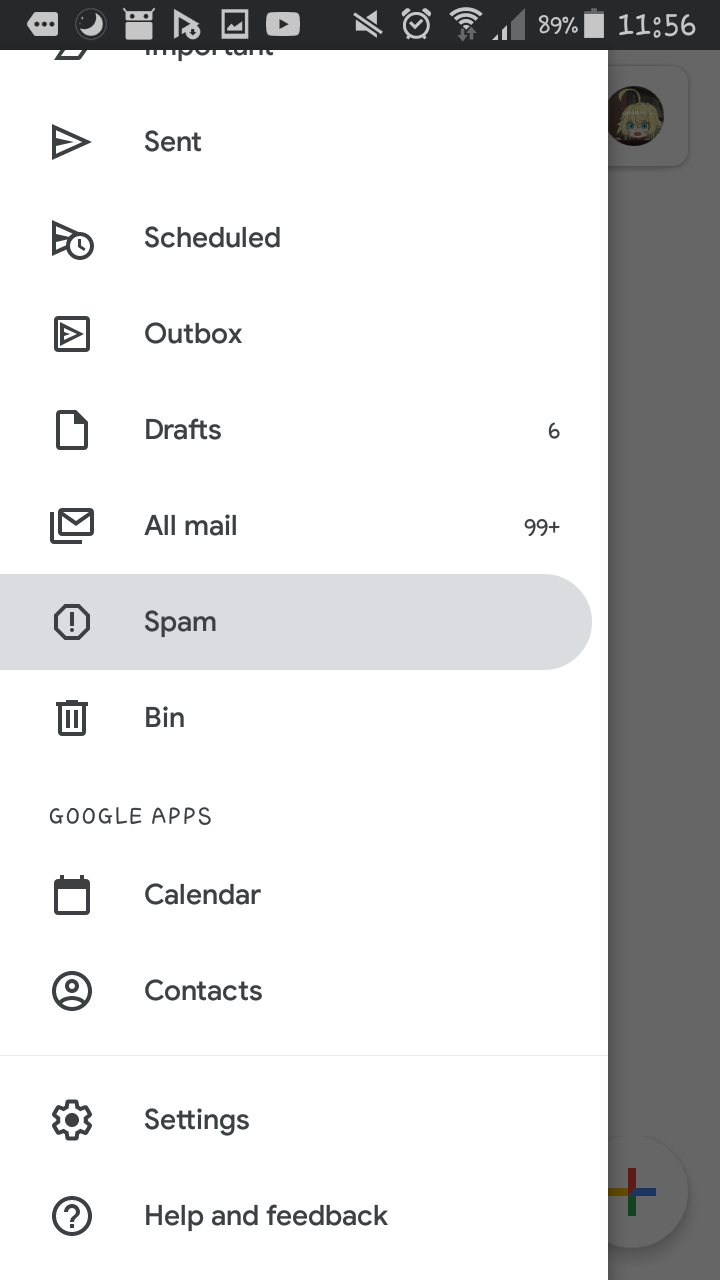
\includegraphics[width=.8\textwidth]{media/gmail-screenshot.png}\\
            \vspace{.5cm}
            
\includegraphics[width=.25\textwidth]{media/gmail-logo.png}
        \end{figure}
    \end{varwidth}
    \hfill
    \begin{varwidth}{.3\textwidth}\pause
        \begin{figure}
        \centering
        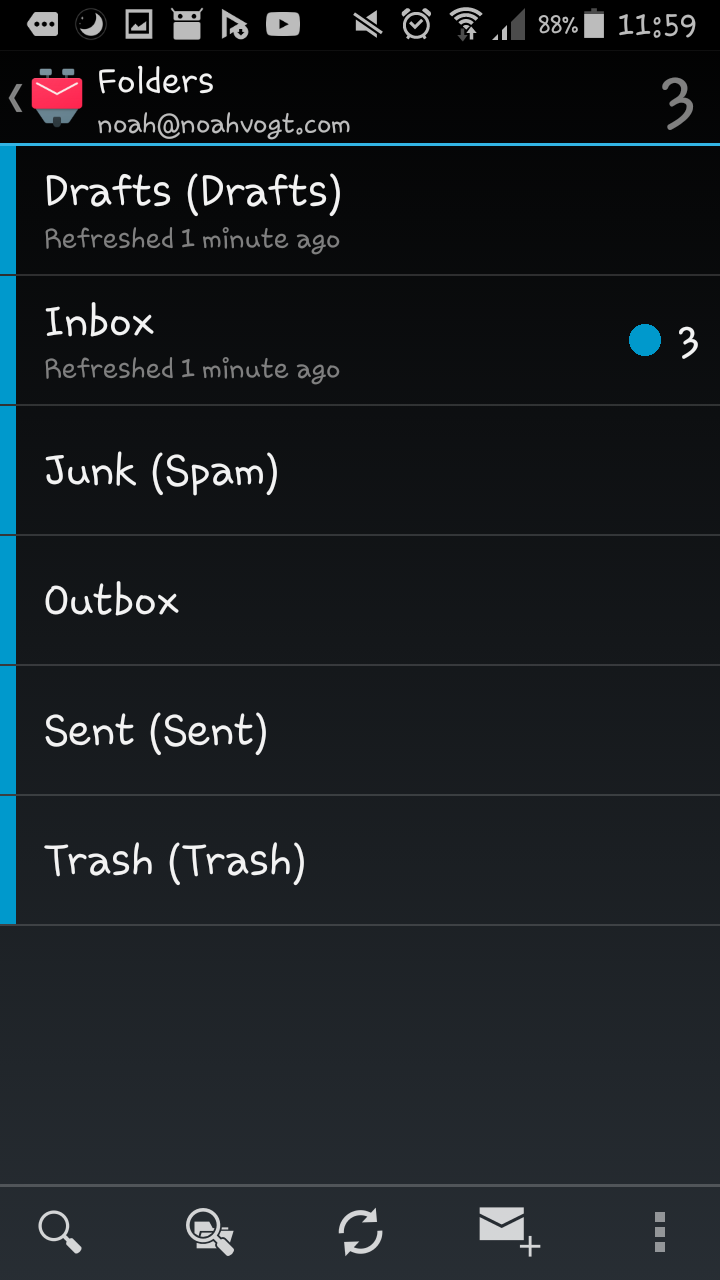
\includegraphics[width=.8\textwidth]{media/k9-screenshot.png}\\
        \vspace{.5cm}
        
\includegraphics[width=.25\textwidth]{media/k9-logo.png}
        \end{figure}
    \end{varwidth}
    \hfill
    \begin{varwidth}{.3\textwidth}\pause
        \begin{figure}
        \centering
        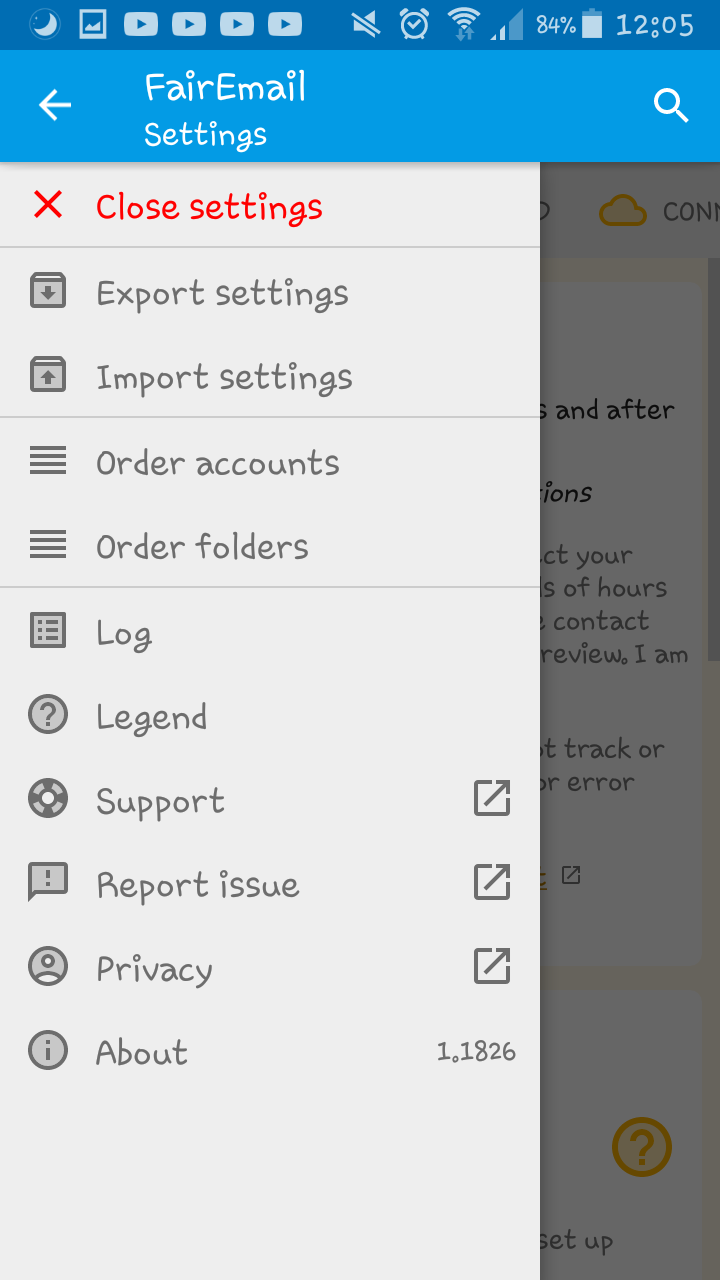
\includegraphics[width=.8\textwidth]{media/fairmail-screenshot.png}\\
        \vspace{.5cm}
        
\includegraphics[width=.25\textwidth]{media/fairmail-logo.png}
        \end{figure}
\end{varwidth}
\end{frame}

% TODO: consider using external player
\section{Haupteil}
\subsection{App mit Film}
\begin{frame}[plain]{Demo}
        \centering
        %\movie[externalviewer]{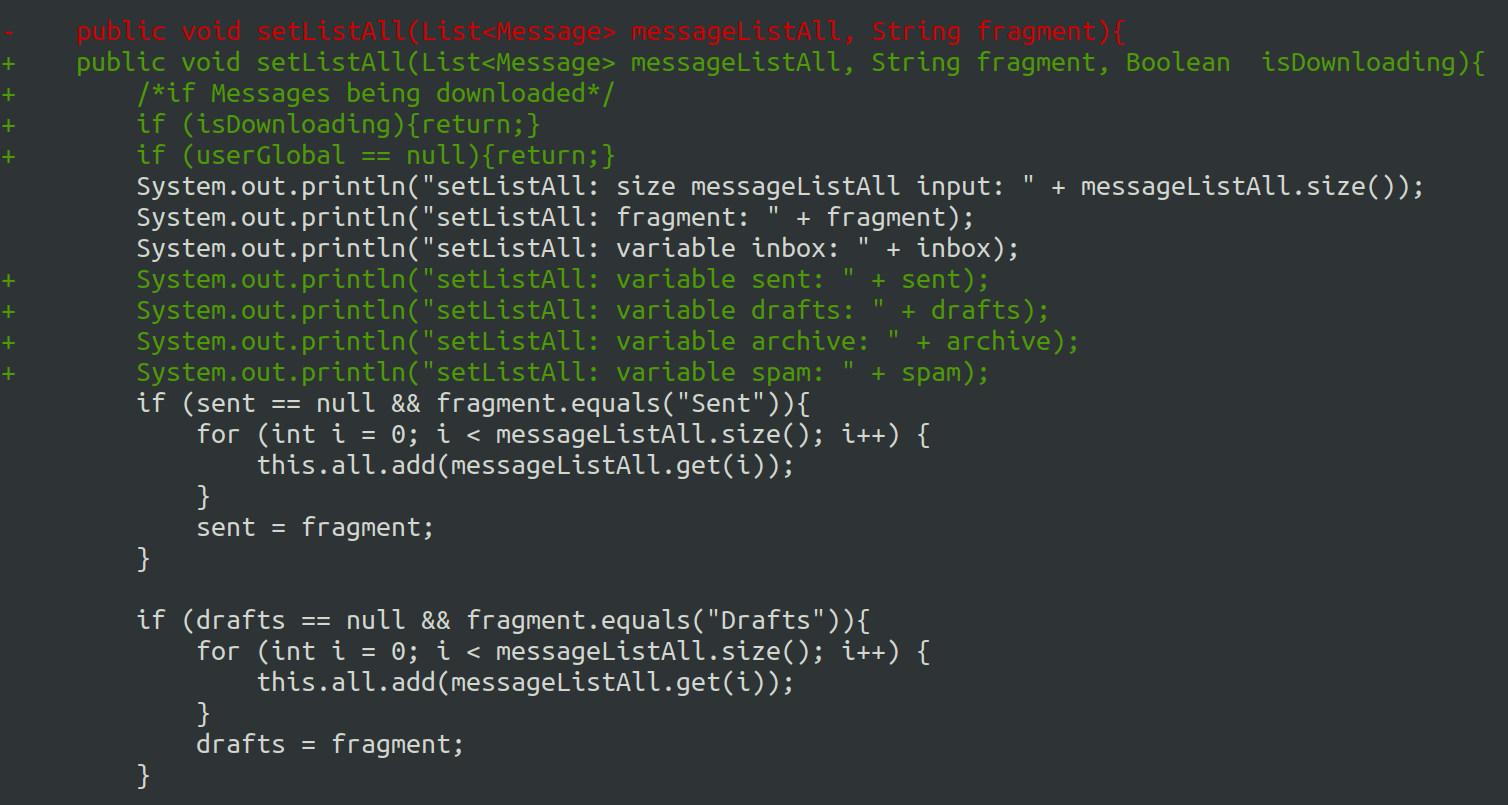
\includegraphics[width=.8\textwidth]{media/bug.png}}{media/appNoSound.mp4}
        %\includemovie[externalviewer, autoplay]{20pt}{20pt}{media/appNoSound.mp4}
%        \includemedia[
%        width=5cm,height=5cm,
%        activate=pageopen,
%        addresource=media/appNoSound.mp4,
%        flashvars={
%            source=media/appNoSound.mp4
%           &autoPlay=true
%           &scaleMode=letterbox
%    }
%]{}{VPlayer.swf}
\end{frame}

\subsection{App Inhalte}
\begin{frame}[plain]{Was alles drin ist}
    \centering
    \begin{figure}[h]
        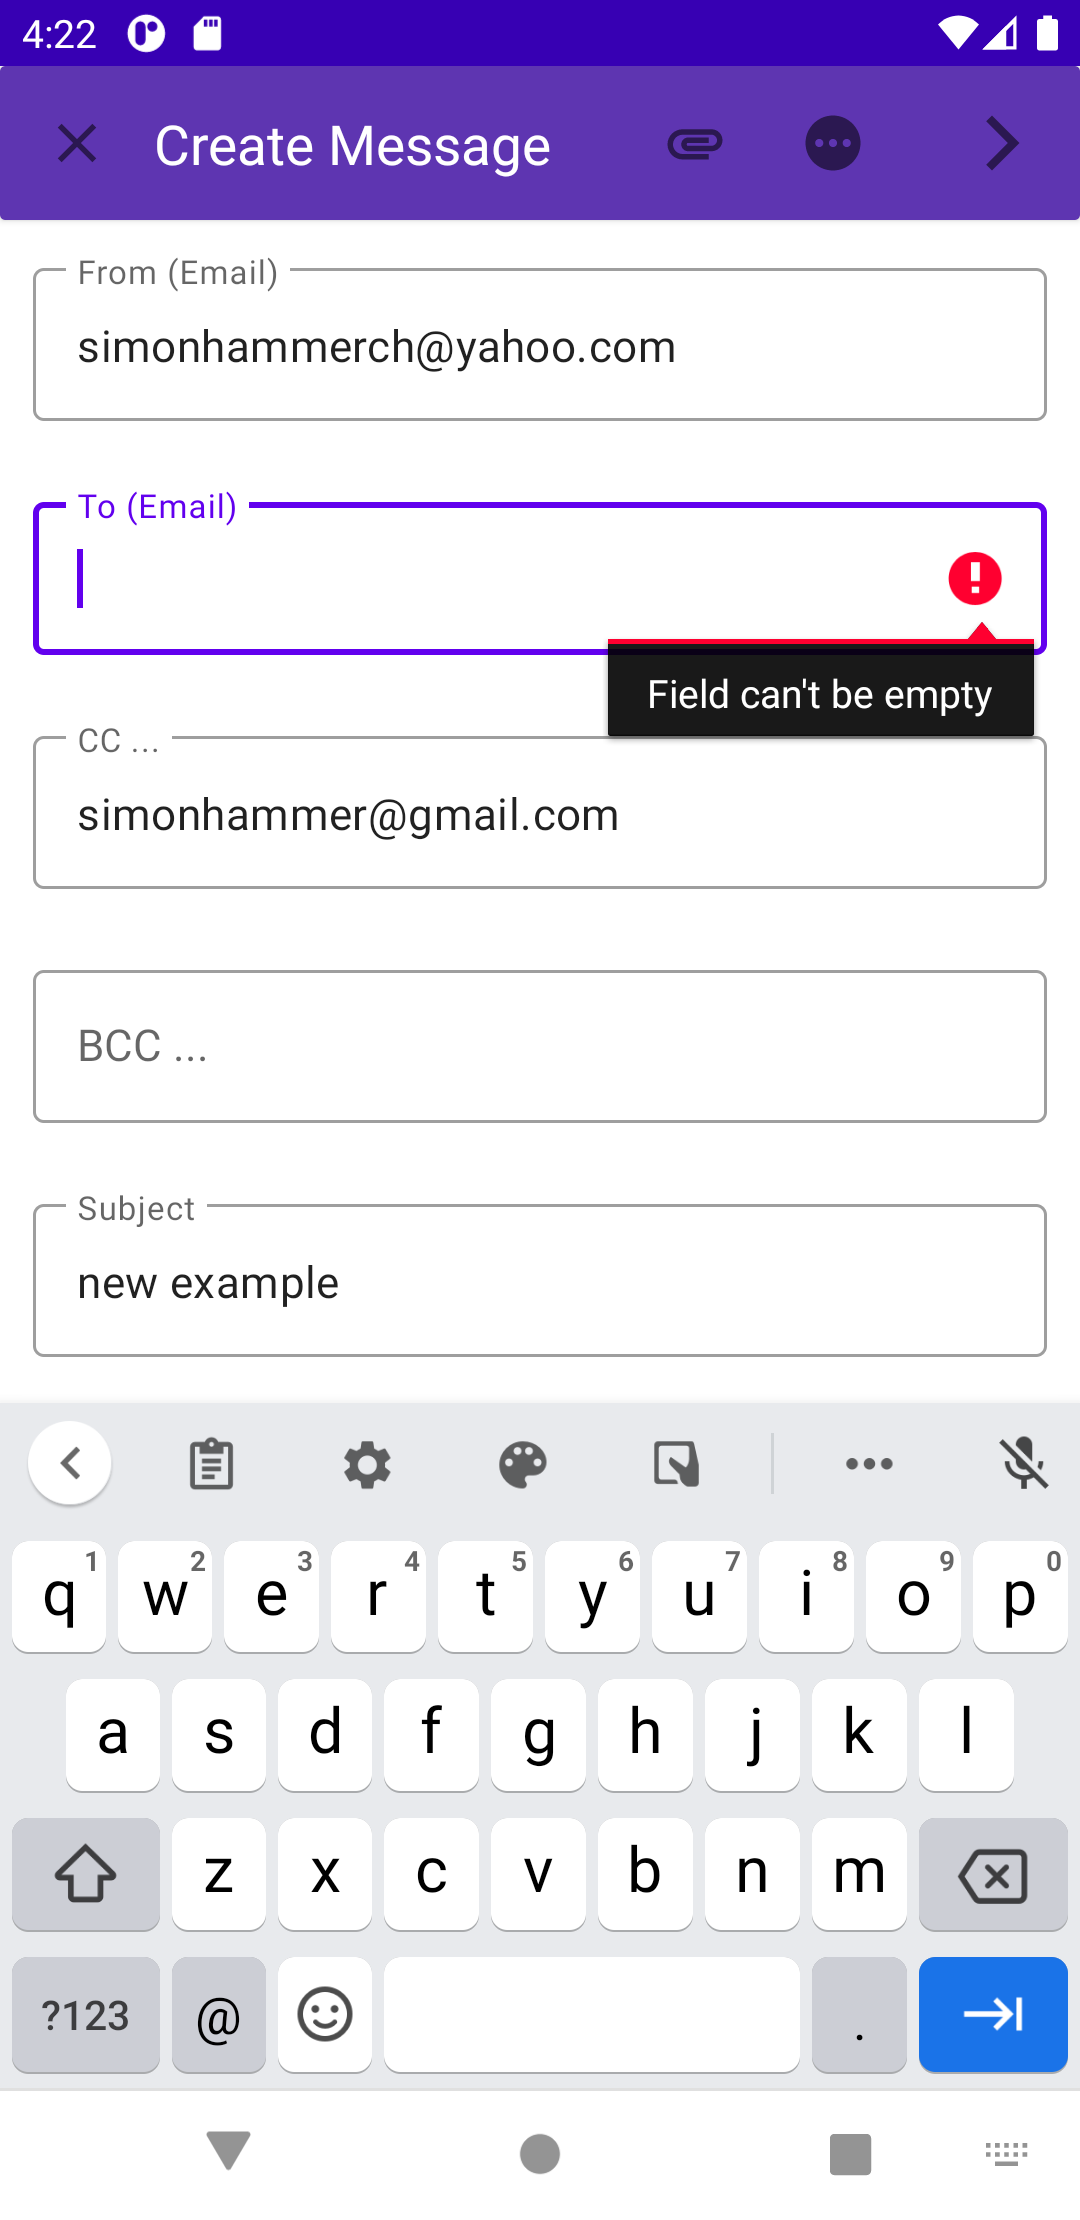
\includegraphics[height=.9\textheight]{media/errorMessage.png}
        \hspace{2.5cm}
        \pause
        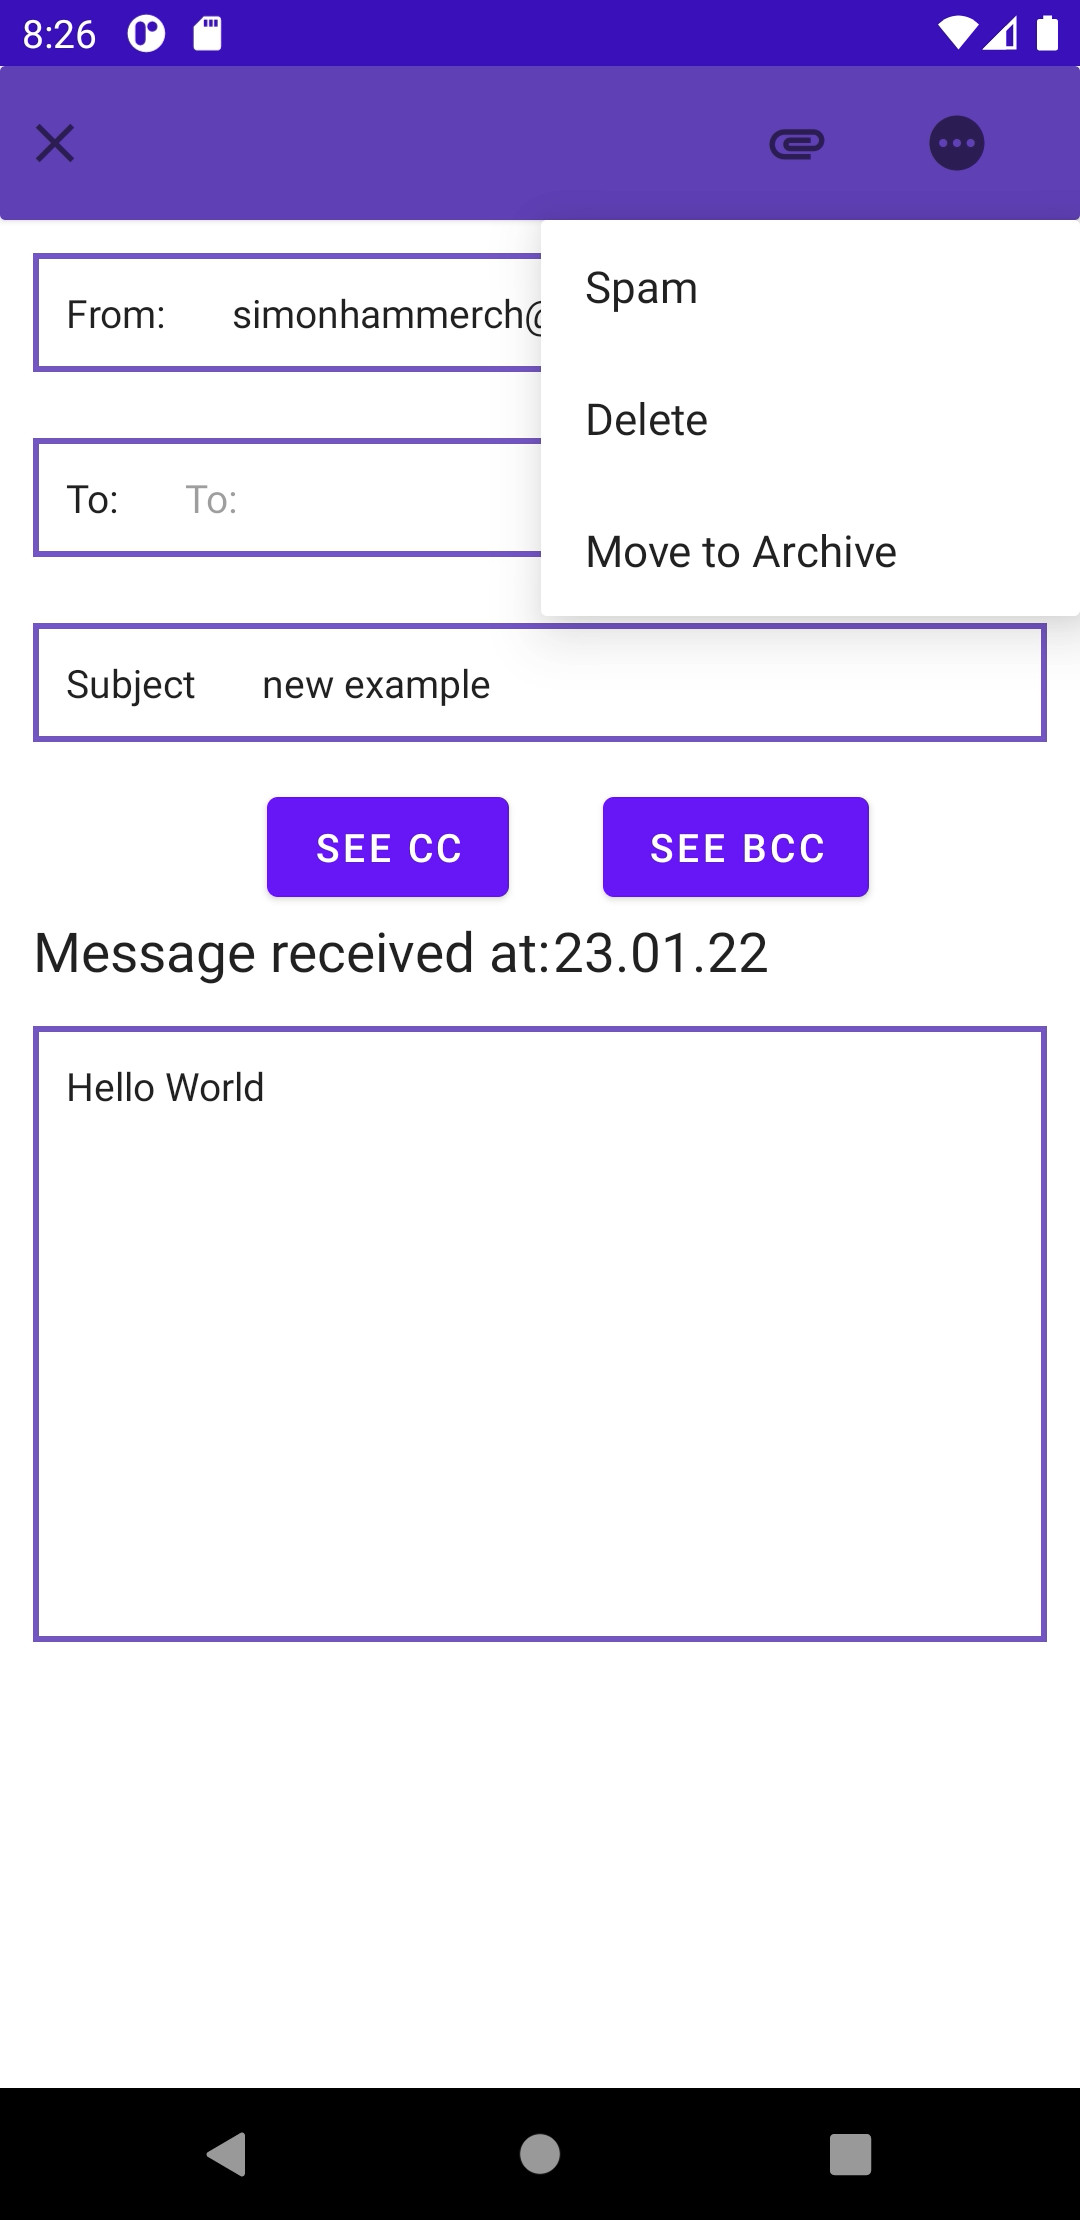
\includegraphics[height=.9\textheight]{media/moreSettings.jpg}
    \end{figure}
\end{frame}

\subsection{App-Struktur}
\begin{frame}[plain]{Allgemeine App-Struktur}
\begin{varwidth}{.3\textwidth}
    \pause
        \begin{figure}
            \centering
            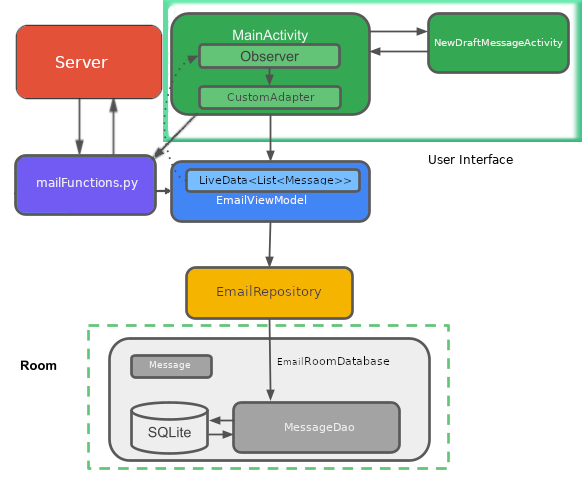
\includegraphics[height=.8\textheight]{../maturText/media/AppStructureFull.png}
        \end{figure}
    \end{varwidth}
    \hfill
    \begin{varwidth}{.5\textwidth}
        \begin{itemize}\pause
            \item User Interface \pause
            \item Server Connection \pause
            \item Database
        \end{itemize}
    \end{varwidth} 
\end{frame}

\begin{frame}[plain]{Database}
\begin{block}{Allgemein}
\textbf{Datenbank:} eine organisierte Ansammlung von strukturierter Information oder Daten
\end{block}

\begin{block}{in Der App}
%:TODO finish this simon
    \pause
\begin{tabular}{ |C{1.4Cm}  |C{0.9Cm} |C{0.5Cm} |C{0.65Cm} |C{0.95Cm} |C{0.85Cm} |C{1.05Cm} |C{1.55Cm} |C{1.05Cm} |C{0.8Cm}|}
%\begin{tabular}{ c c c c c c c c c c}
 \hline
 \multicolumn{10}{|c|}{Database Table} \\
 \hline
    \small{ObejctKey} &To & cc & bcc & from & date & subject & \small{textContent} & folder & seen  \\
    \hline
    \pause
     01    & \small{Sam} & null & null & \small{Anna} & \small{1.3.13} & Schule &  Hallo Herr & Draft & true \\
 \hline
\end{tabular} 
\end{block}
\end{frame}

\begin{frame}[plain]{Mail Server Connection}
    \centering
    
\includegraphics[height=.8\textheight]{media/empty.png}
\end{frame}

\begin{frame}[plain]{Mail Server Connection}
    \centering
    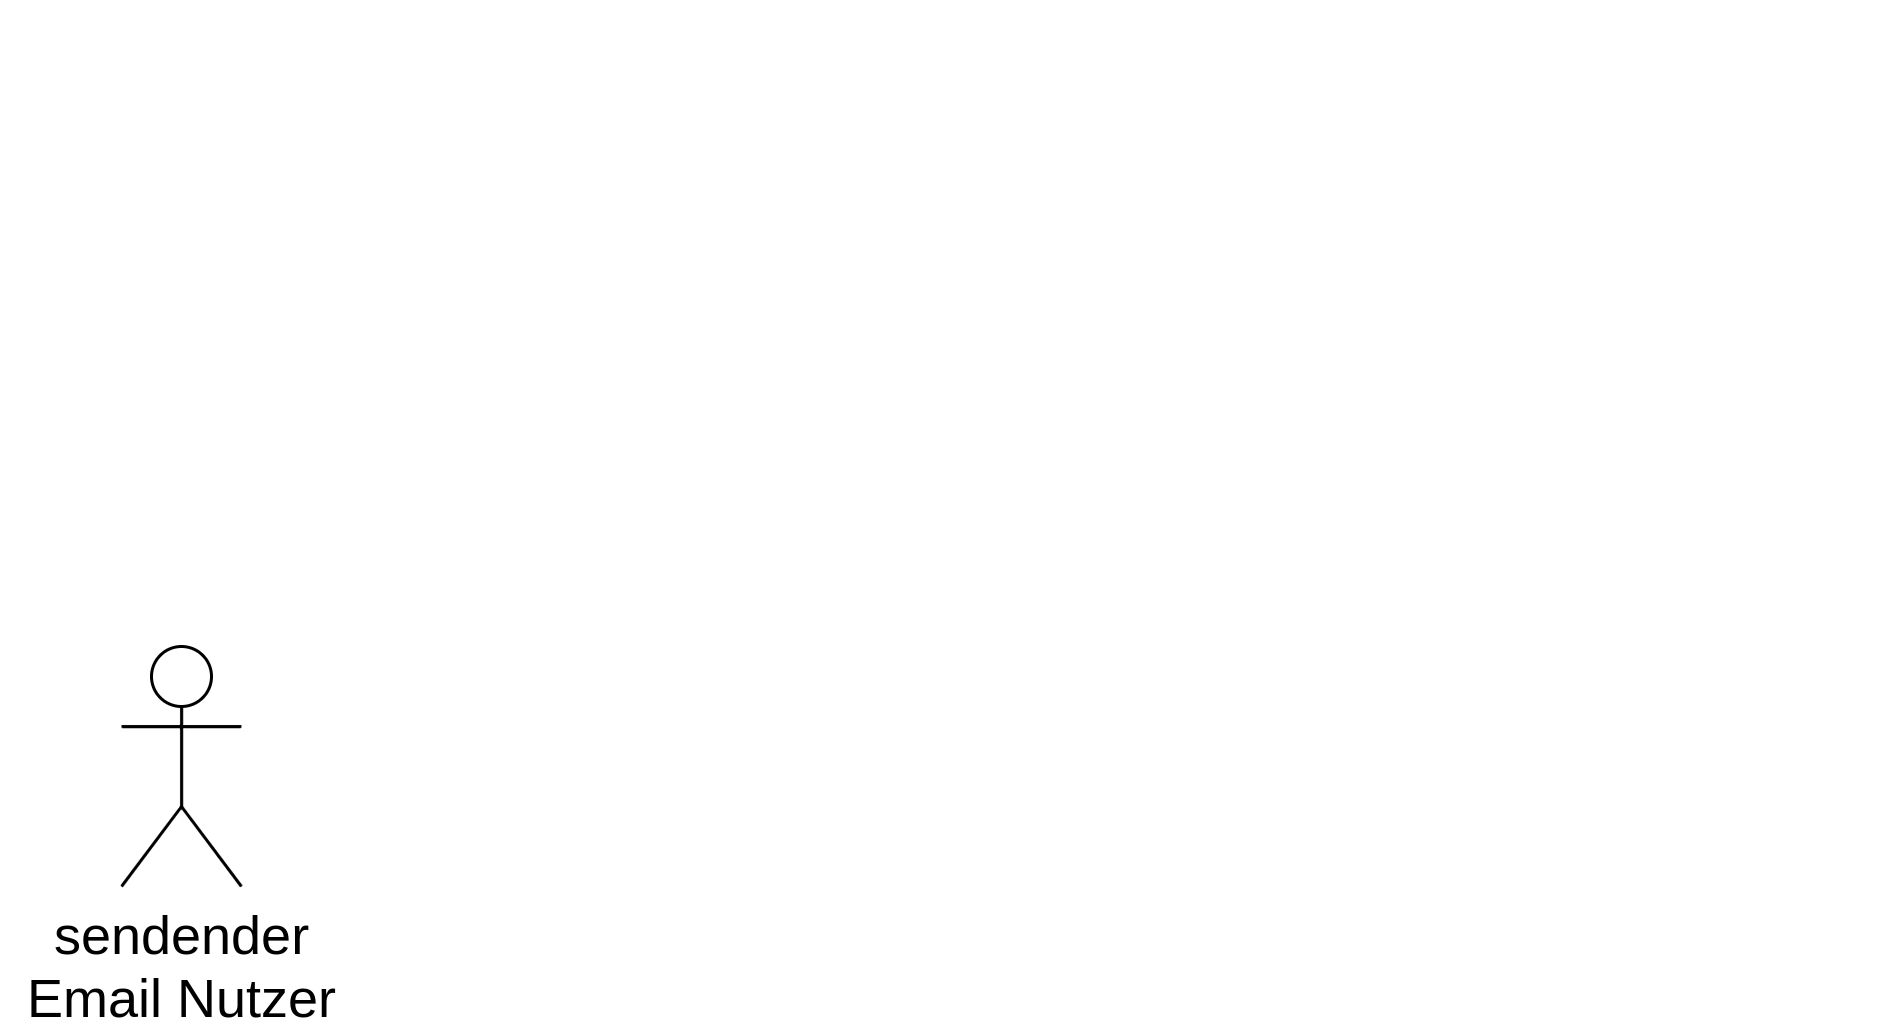
\includegraphics[height=.8\textheight]{media/mail-diagram-01.png}
\end{frame}

\begin{frame}[plain]{Mail Server Connection}
    \centering
    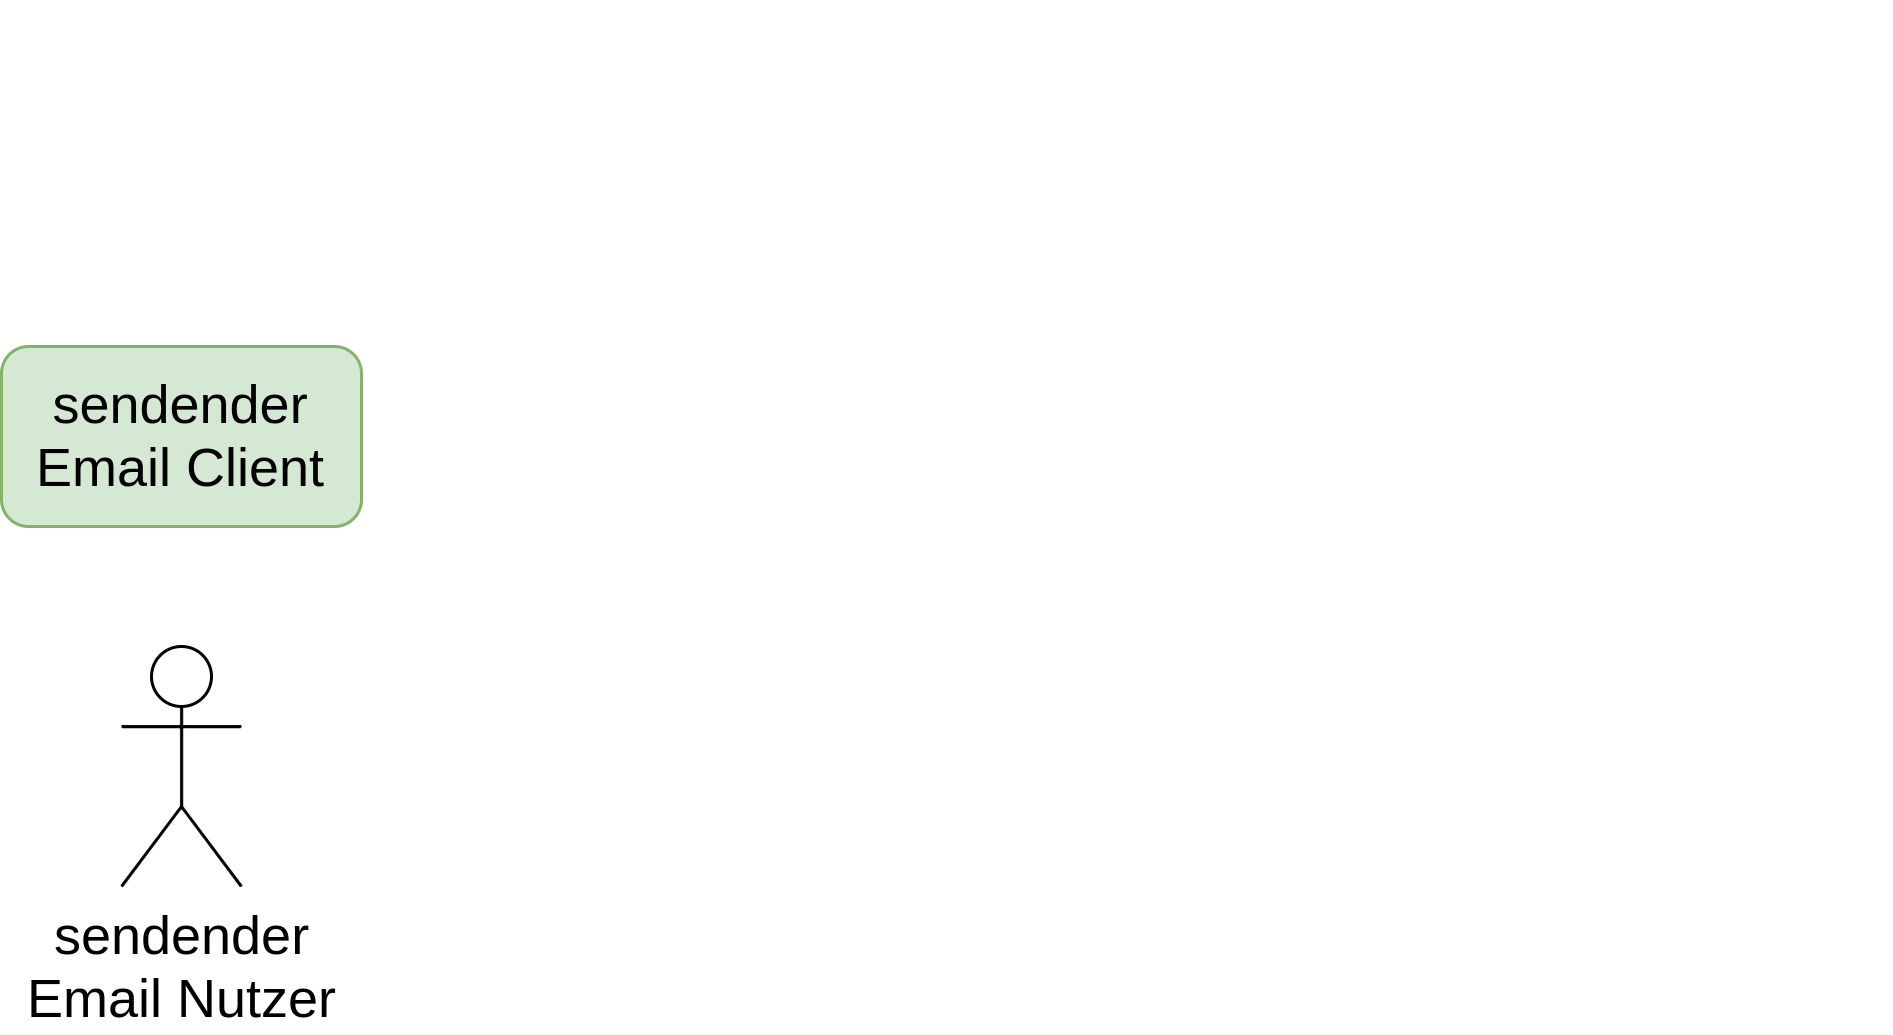
\includegraphics[height=.8\textheight]{media/mail-diagram-02.png}
\end{frame}

\begin{frame}[plain]{Mail Server Connection}
    \centering
    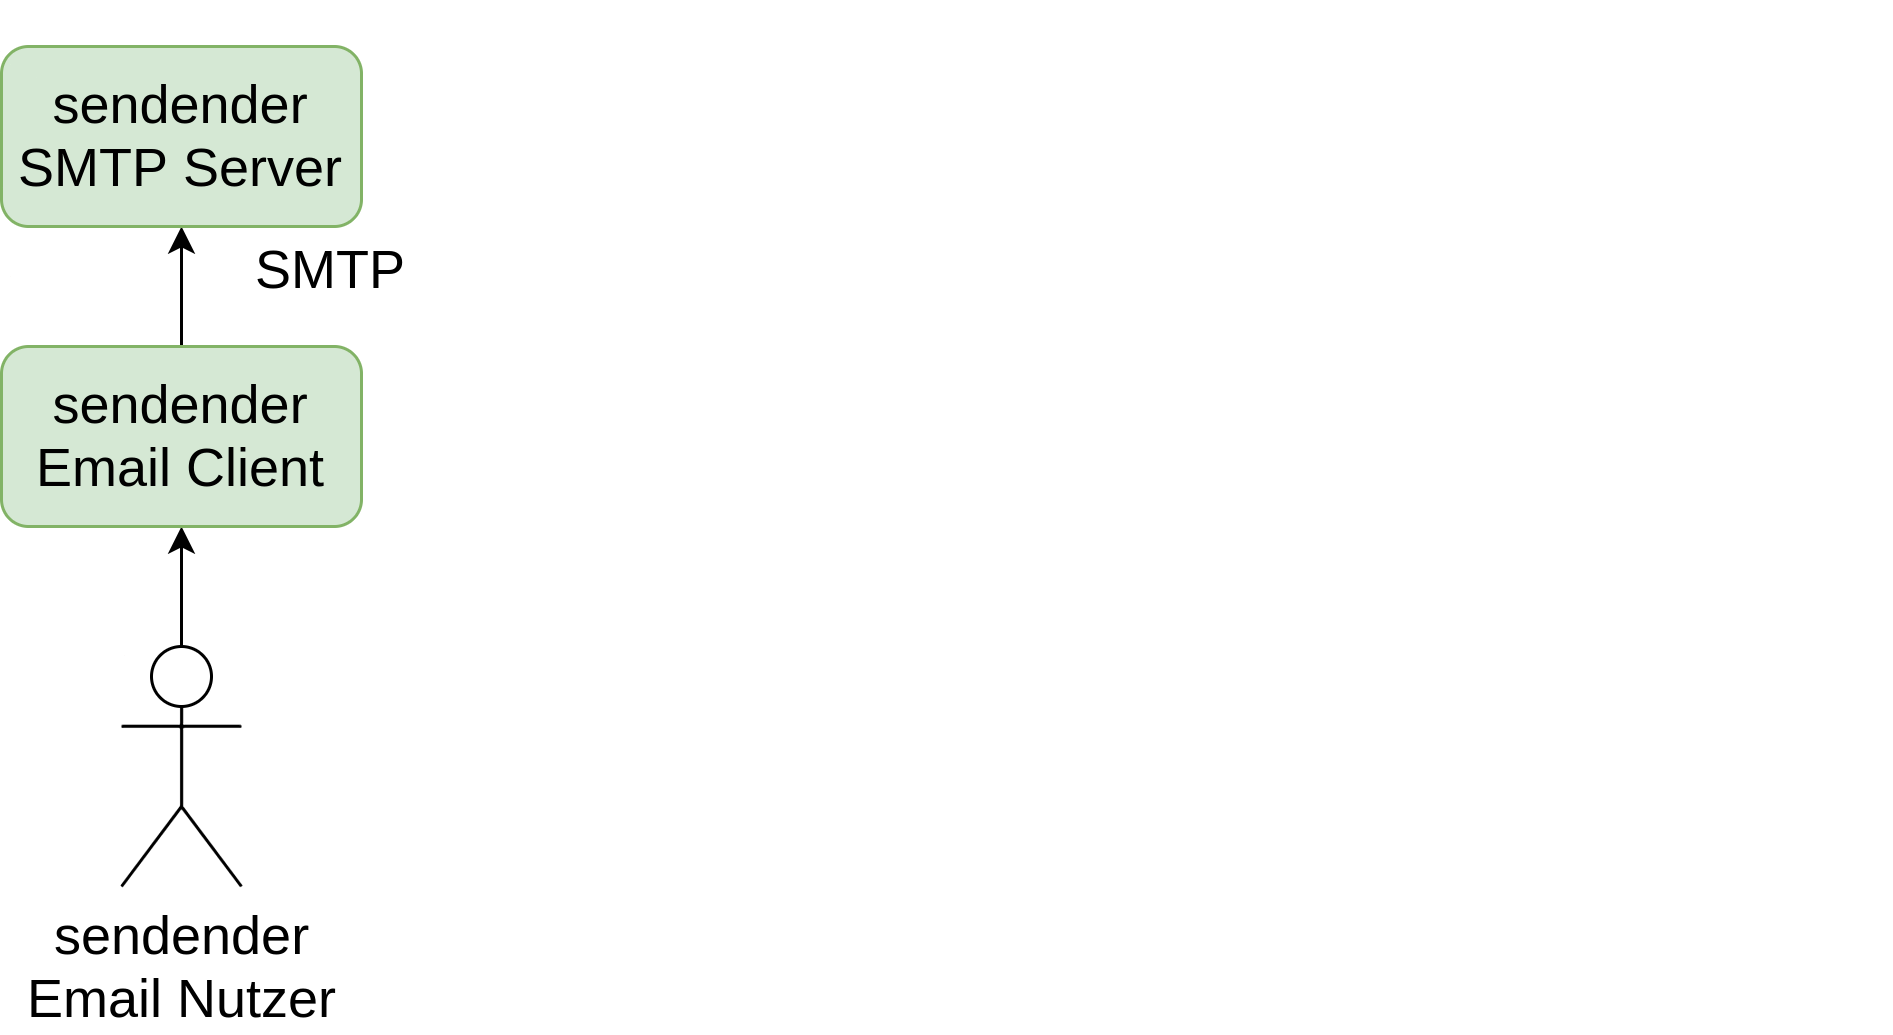
\includegraphics[height=.8\textheight]{media/mail-diagram-03.png}
\end{frame}

\begin{frame}[plain]{Mail Server Connection}
    \centering
    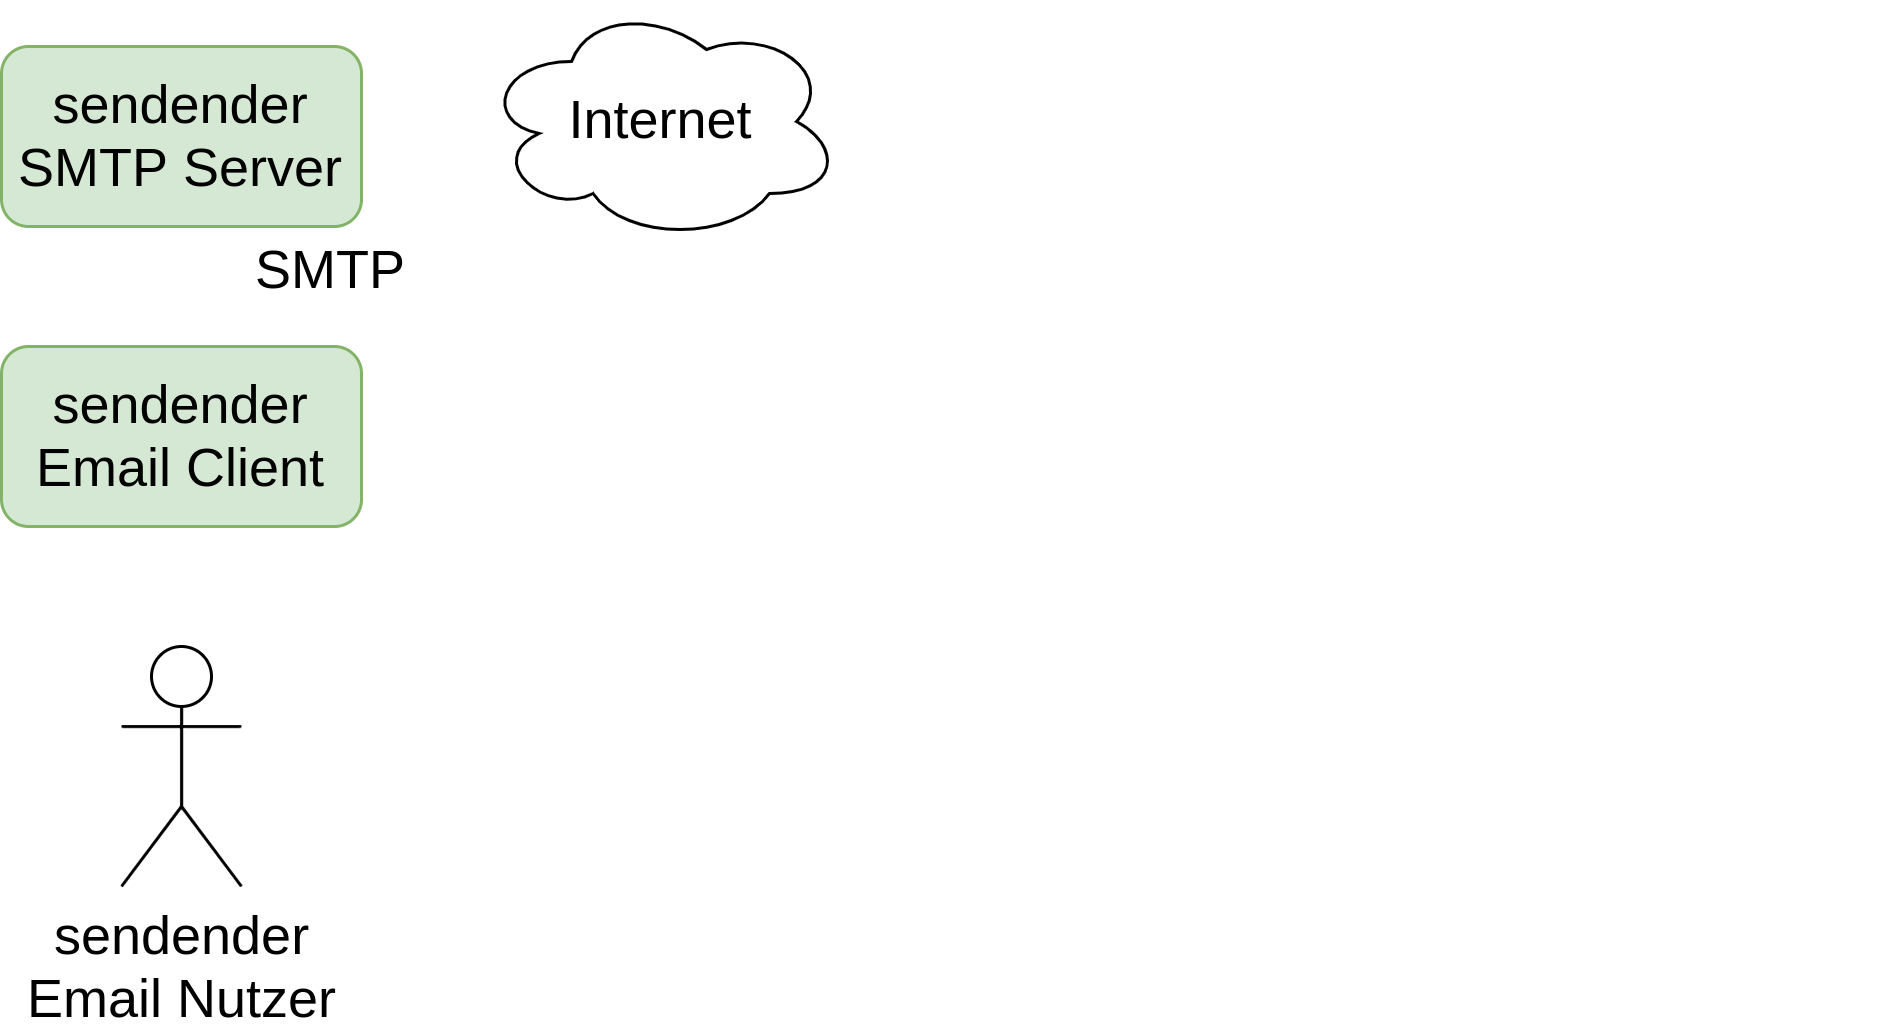
\includegraphics[height=.8\textheight]{media/mail-diagram-04.png}
\end{frame}

\begin{frame}[plain]{Mail Server Connection}
    \centering
    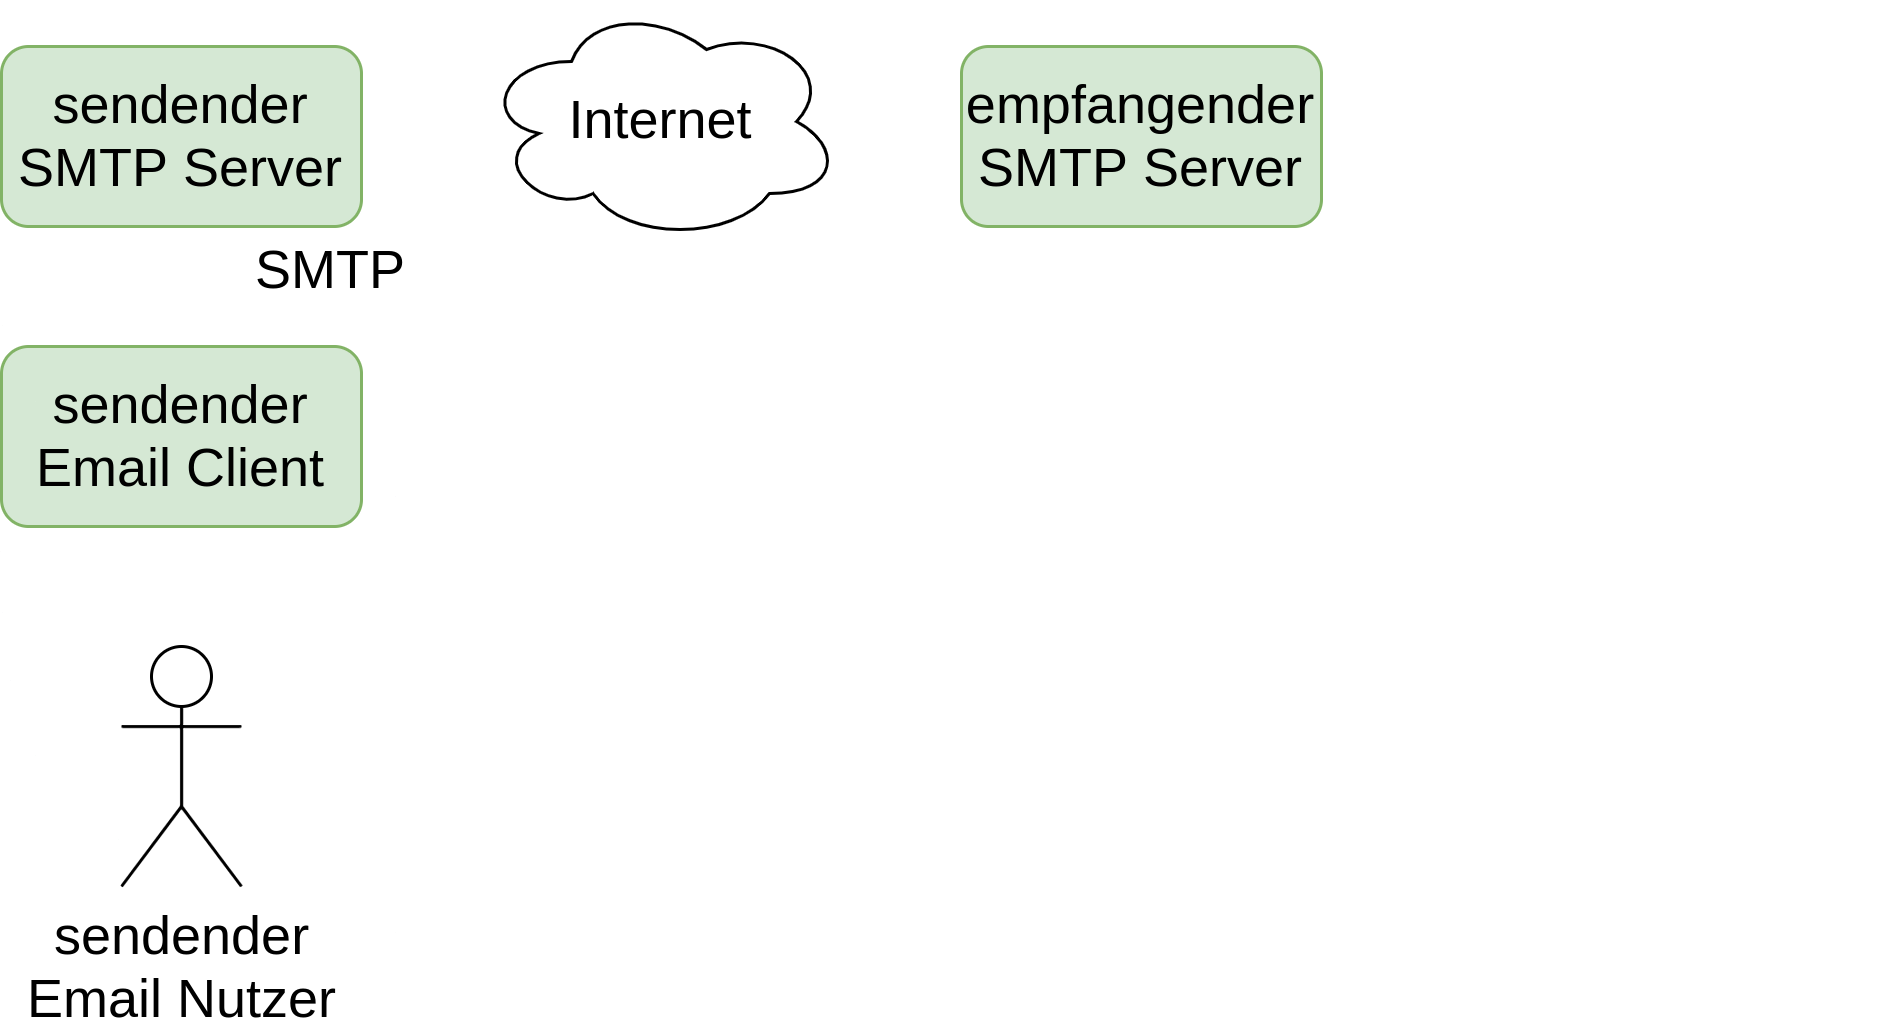
\includegraphics[height=.8\textheight]{media/mail-diagram-05.png}
\end{frame}

\begin{frame}[plain]{Mail Server Connection}
    \centering
    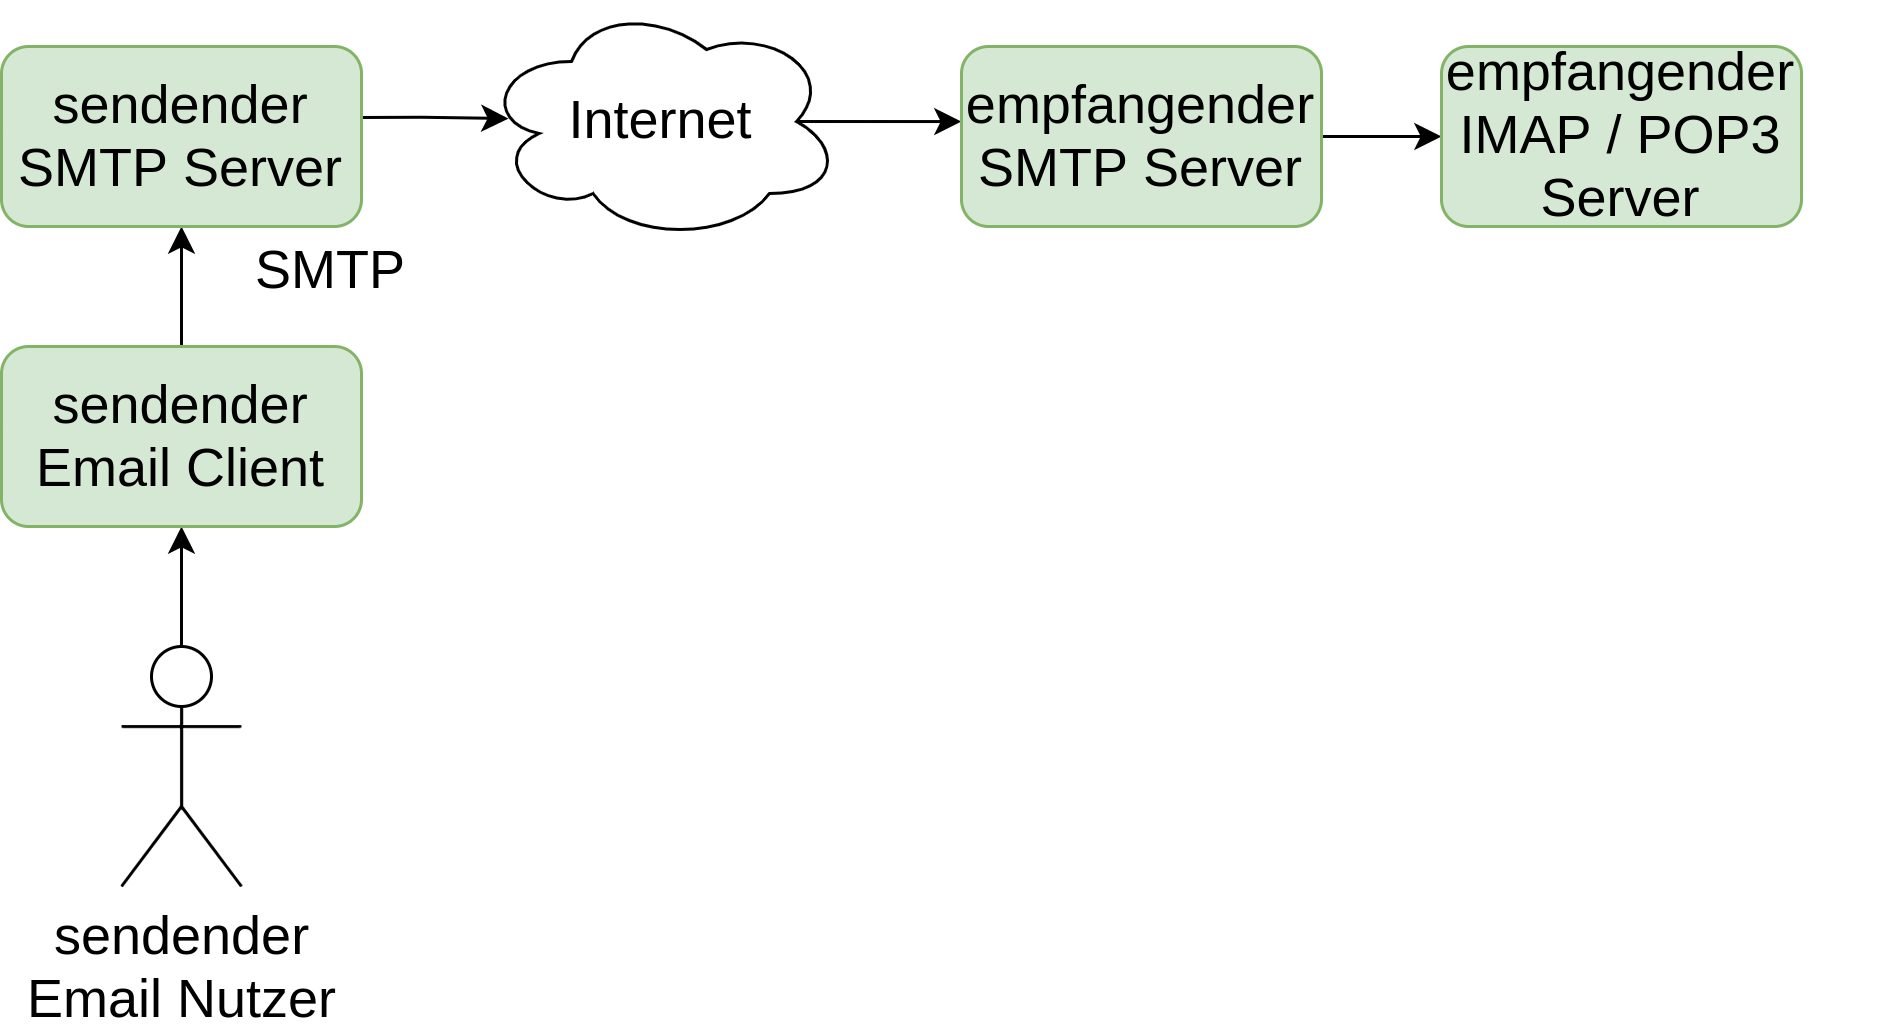
\includegraphics[height=.8\textheight]{media/mail-diagram-06.png}
\end{frame}

\begin{frame}[plain]{Mail Server Connection}
    \centering
    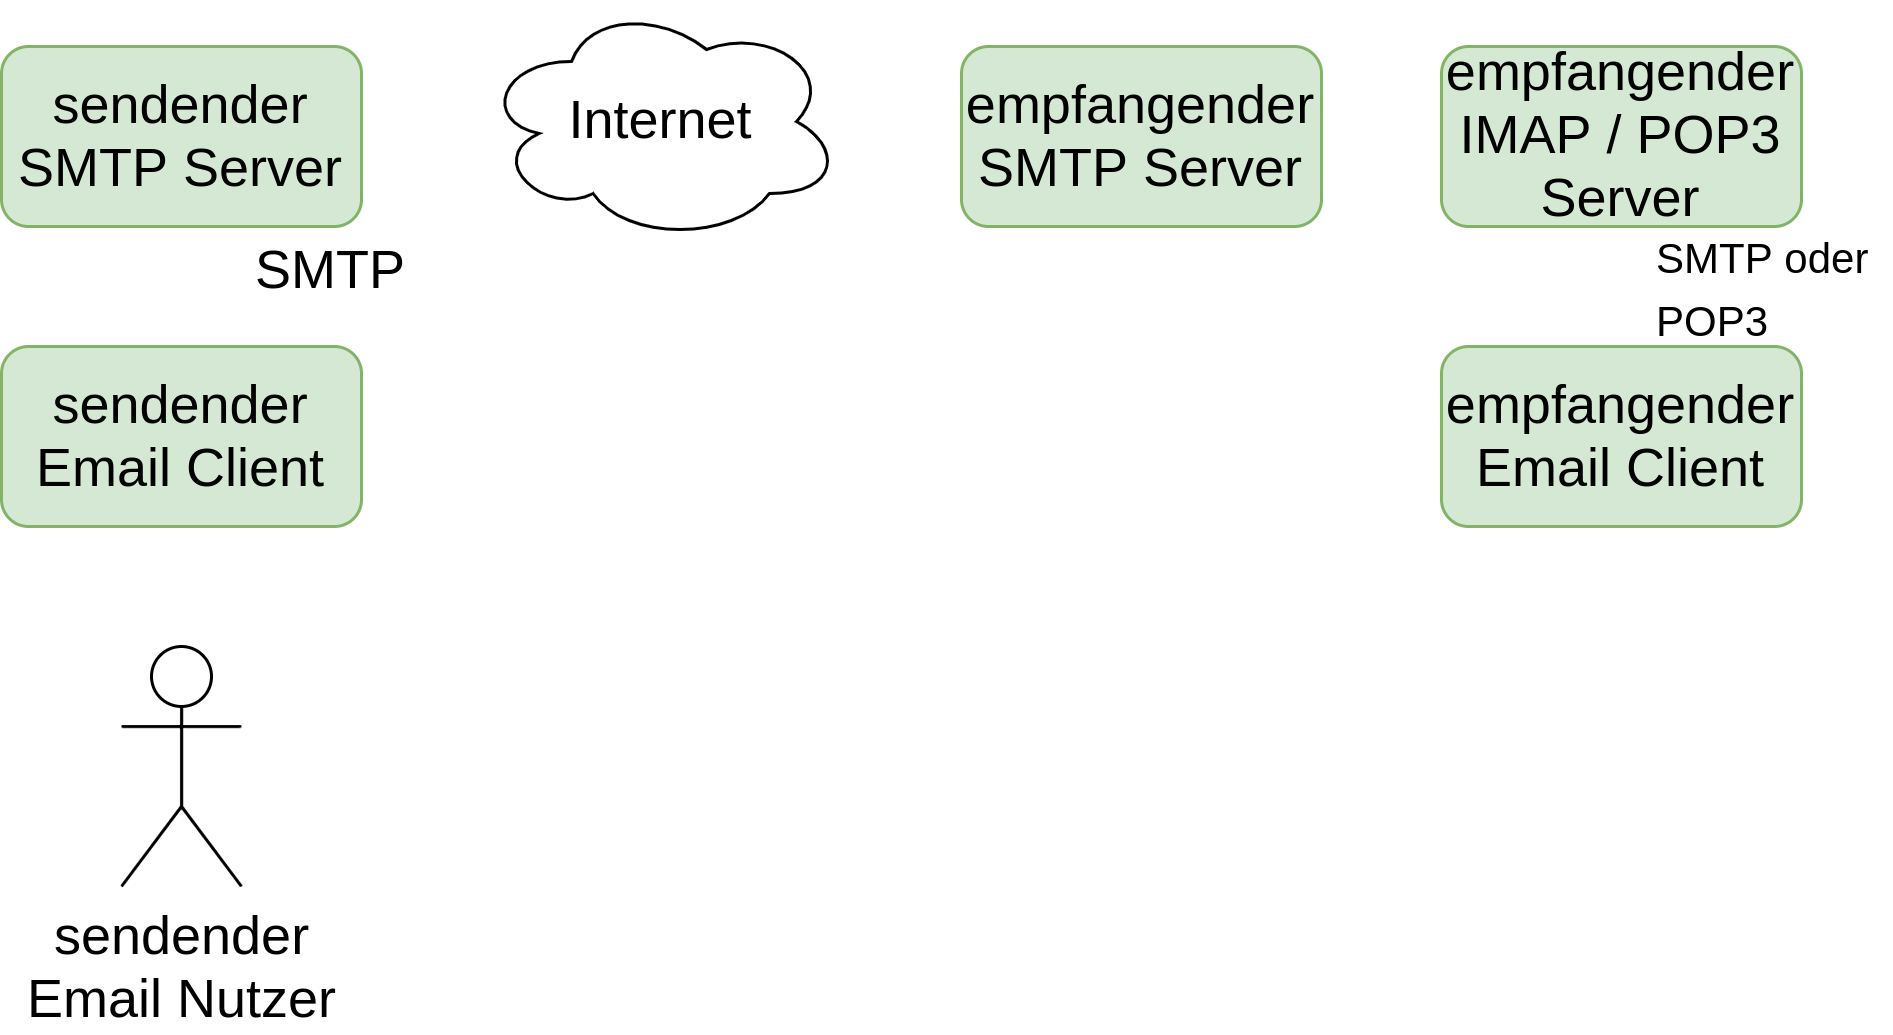
\includegraphics[height=.8\textheight]{media/mail-diagram-07.png}
\end{frame}

\begin{frame}[plain]{Mail Server Connection}
    \centering
    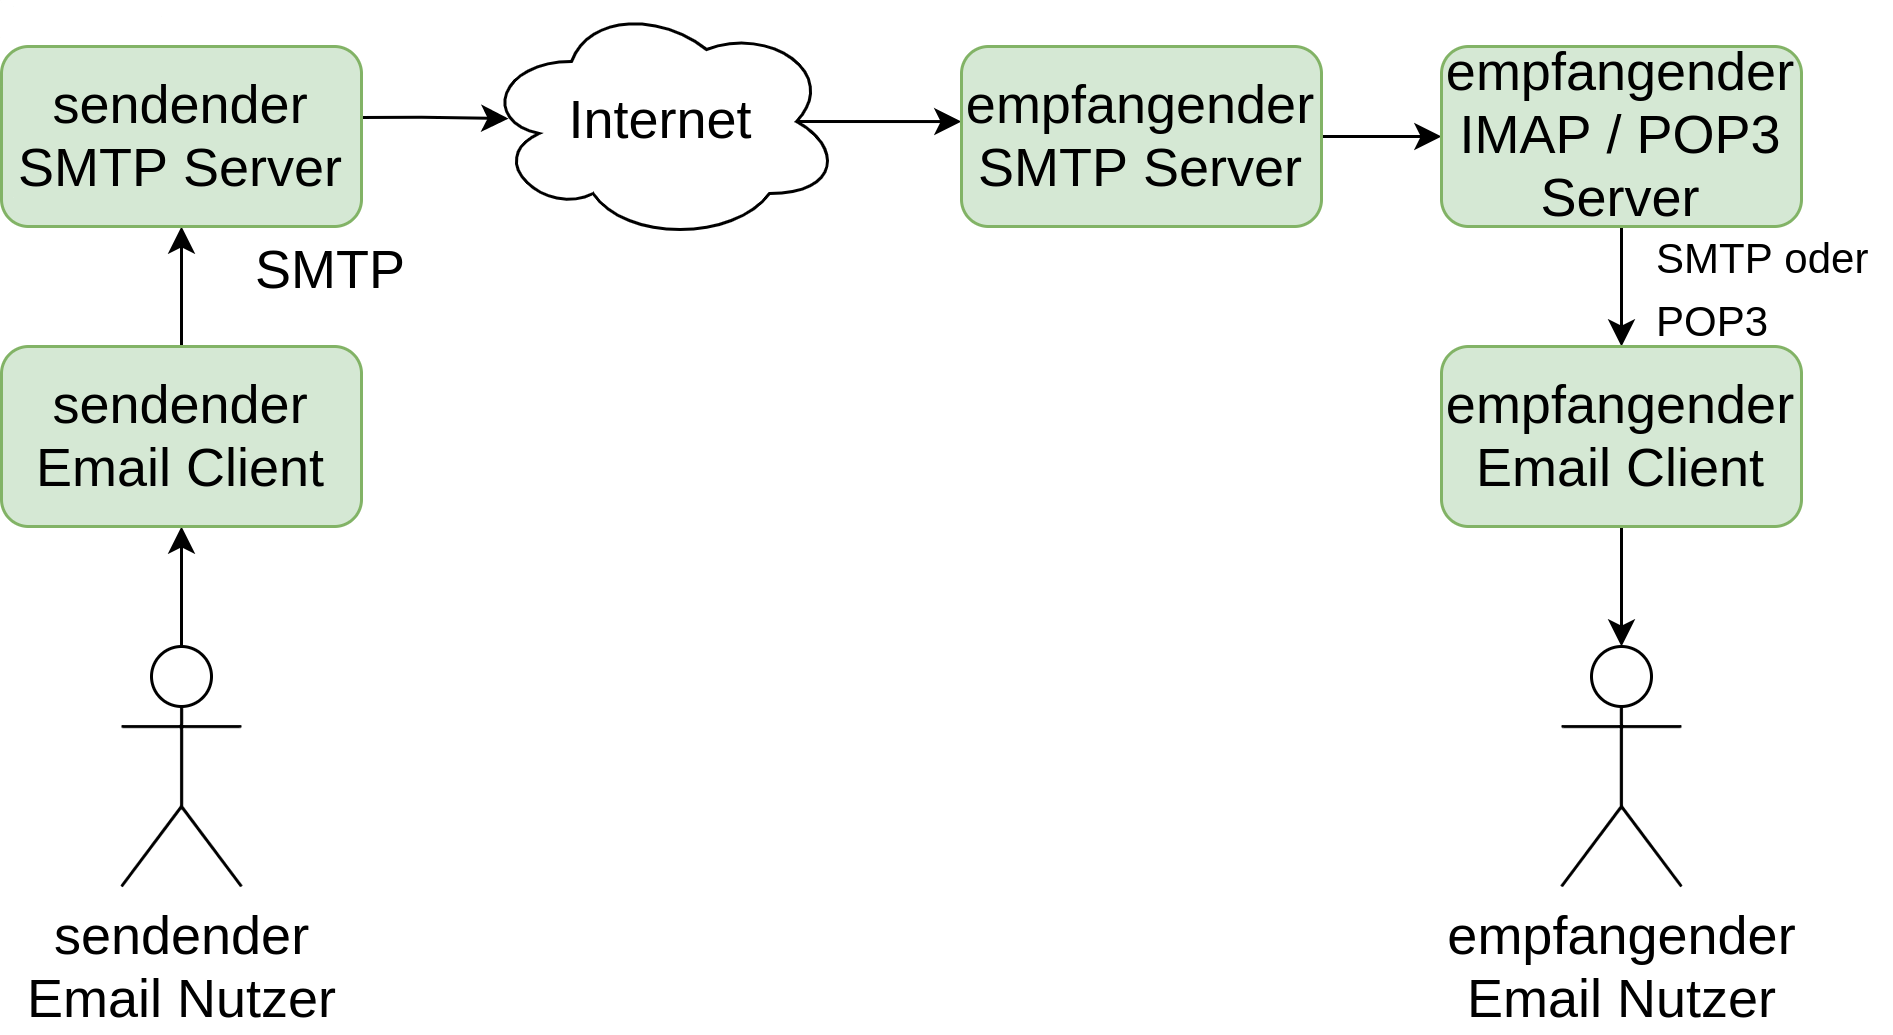
\includegraphics[height=.8\textheight]{media/mail-diagram-08.png}
\end{frame}
% TODO: not use lstlisting?
\defverbatim[colored]\makeset{
\lstset{language=python}
\begin{lstlisting}
def sendStarttls(host, sendingMail, receivingMail, password, message="",
                 subject="", port=587, cc=[], bcc=[]):
    context = ssl.create_default_context()

    if type(cc) is not str:
        cc = ",".join(cc)
    if type(bcc) is not str:
        bcc = ",".join(bcc)
    utf8Message = ("Subject: " + subject + "\nCC: " + cc + "\nBCC: " + bcc +
                   "\n\n" + message)
    decoded = utf8Message.encode('cp1252').decode('utf-8')

    with smtplib.SMTP(host, port) as serverConnection:
        serverConnection.starttls(context=context)
        serverConnection.login(sendingMail, password)
        serverConnection.sendmail(sendingMail, receivingMail, decoded)
\end{lstlisting}
}


\begin{frame}[plain]{Senden einer Email}
%\makeset
    %\lstset{language=Python}
    %\lstinputlisting[language=Python]{code/sentMail.py}
    \begin{figure}[h]
        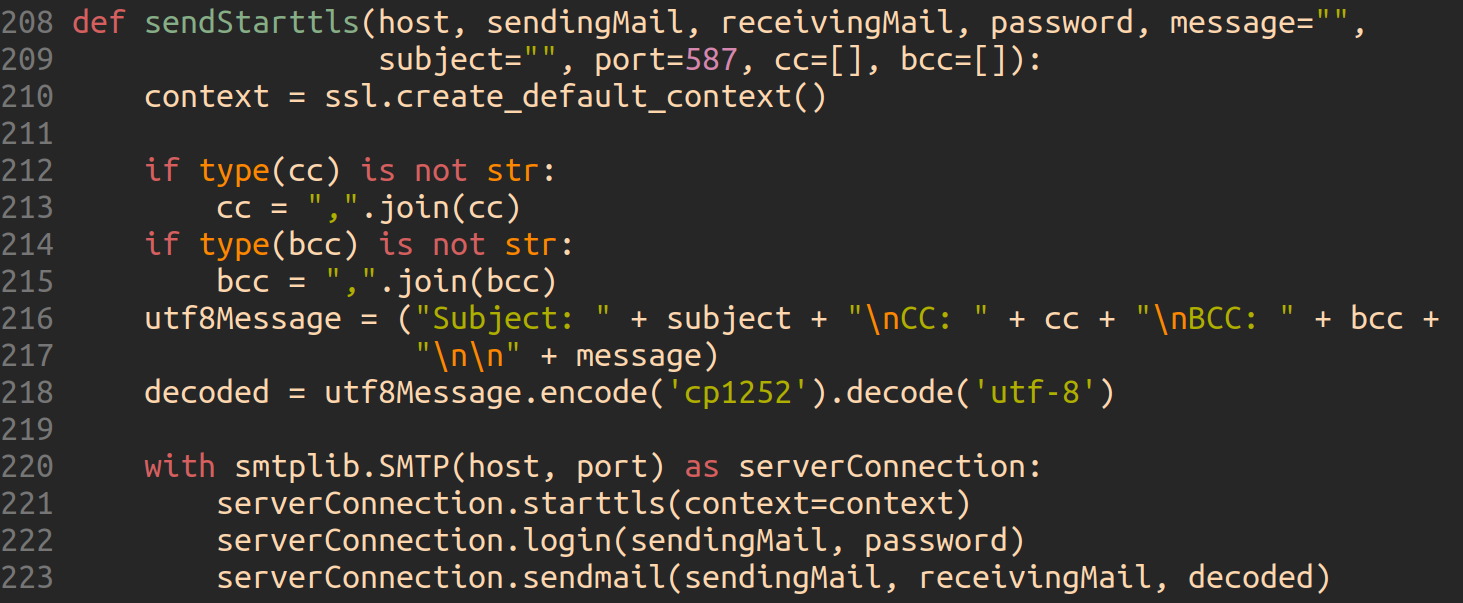
\includegraphics[width=.8\textwidth]{media/codeFragment.png}
    \end{figure}
\end{frame}


\subsection{Librarys}
\begin{frame}[plain]{Material Design}
\begin{varwidth}{.5\textwidth}
        \begin{figure}
            \centering
            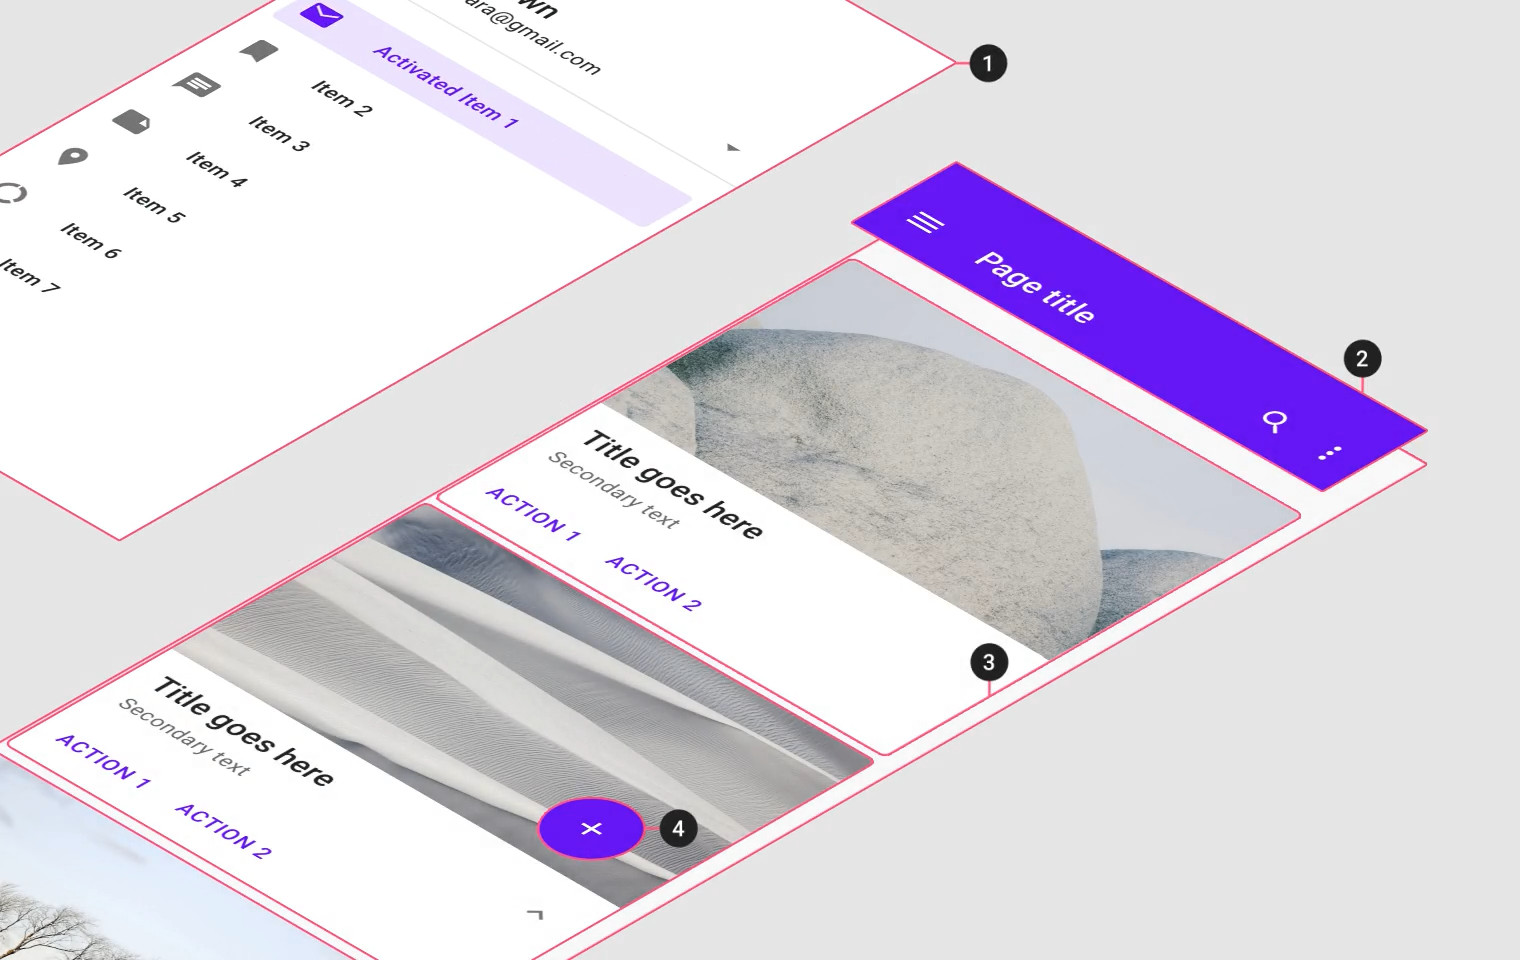
\includegraphics[width=\textwidth]{media/material-design-in-action.jpg}
        \end{figure}
    \end{varwidth}
    \hfill
    \begin{varwidth}{.4\textwidth}
        
\includegraphics[width=\textwidth]{media/material-android.png}
        \begin{itemize}\pause
            \item GUI-Framework\pause
            \item beliebt\pause
            \item in Google Apps
        \end{itemize}
    \end{varwidth}
\end{frame}

% TODO: insert bugs
\begin{frame}[plain]{Bugs}
    \begin{figure}[h]
        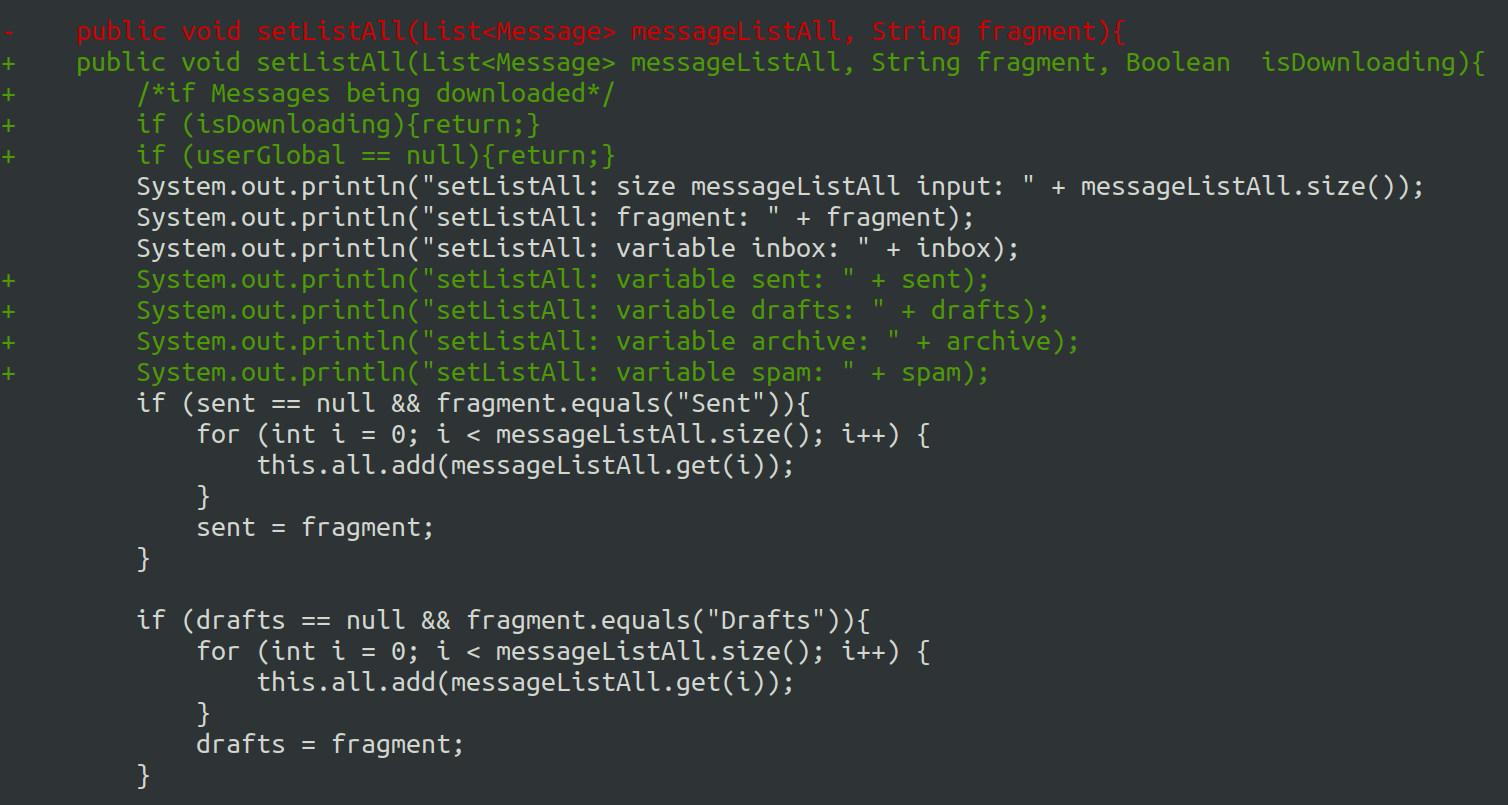
\includegraphics[width=.8\textwidth]{media/bug.png}
    \end{figure}
\end{frame}


\section{Resultate}
\begin{frame}[plain]{Resultate}
\begin{itemize}\pause
    \item User Interface\pause
    \item chaquopy\pause
    \item Funktionalität\pause
    \item abschliessend
\end{itemize}
\end{frame}

\section{Gelerntes}
\begin{frame}[plain]{Was wir gelernt haben}
\begin{varwidth}{.5\textwidth}
        \begin{figure}
            \centering
            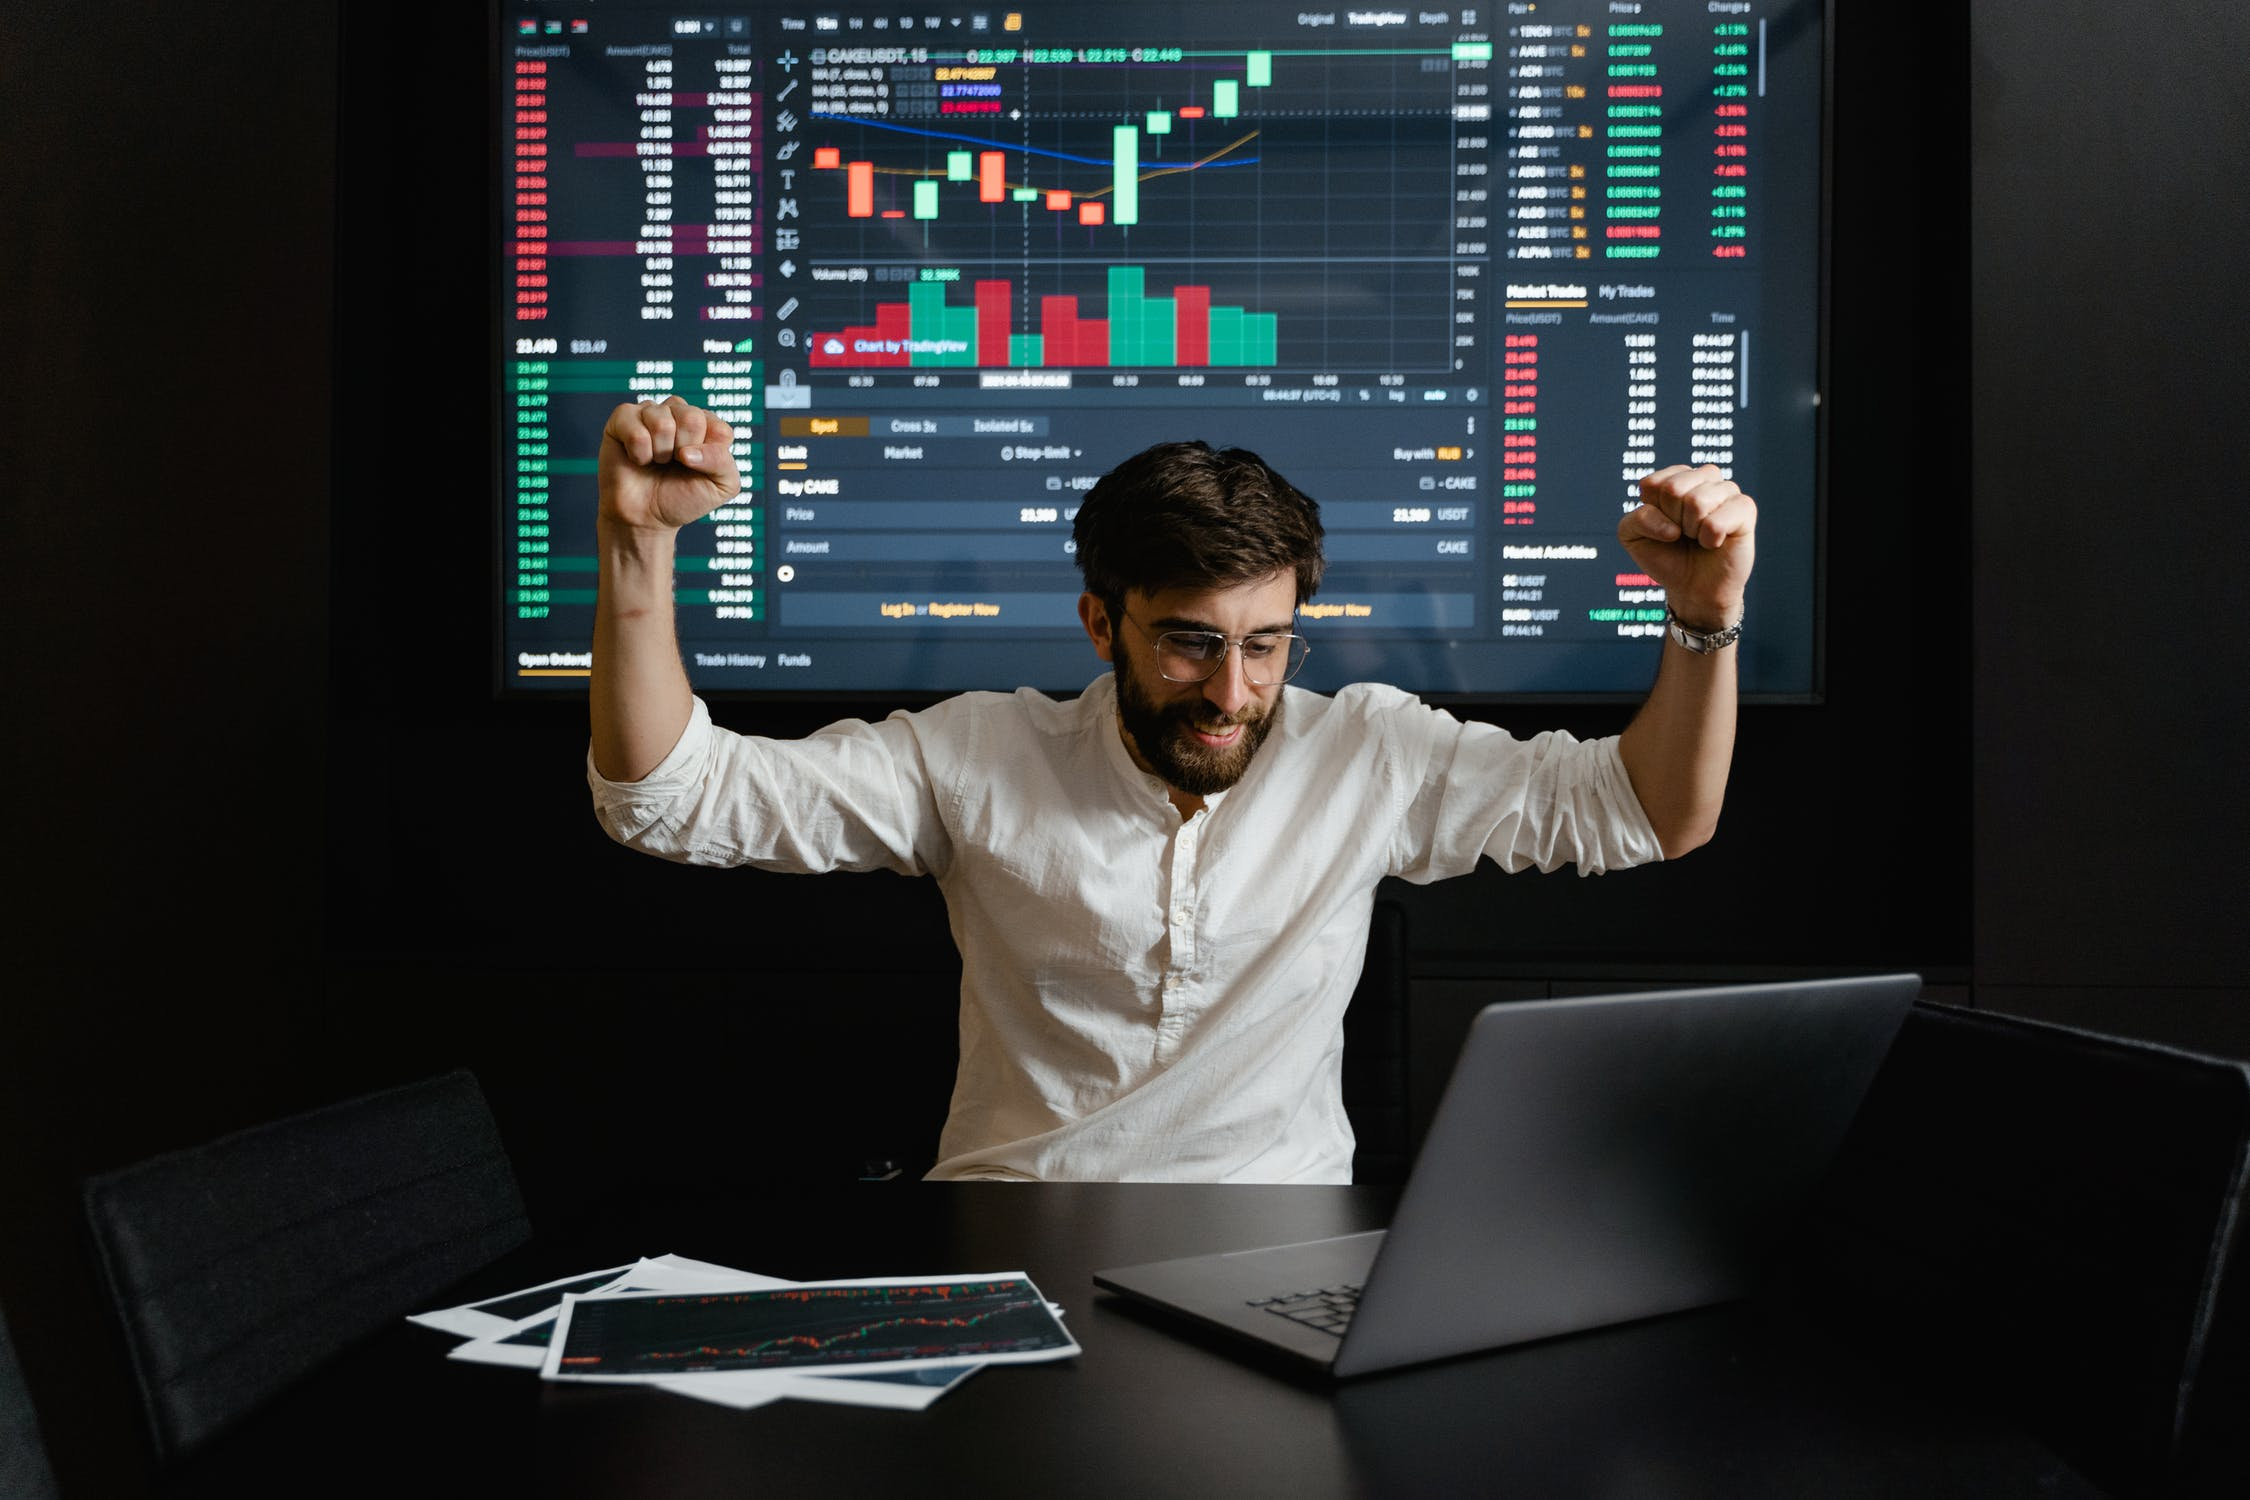
\includegraphics[width=.95\textwidth]{media/monetary-success.jpeg}
        \end{figure}
    \end{varwidth}
    \hfill
    \begin{varwidth}{.5\textwidth}
        \begin{itemize}\pause
            \item Java\inlinegraphics{media/java-only-logo.png}\pause
            \item Android Apps\inlinegraphics{media/android-robot.png}\pause
            \item Android Studio\inlinegraphics{media/android-studio-logo.png}\pause
            \item Database \& SQL\inlinegraphics{media/database.png}\pause
            \item Gradle\inlinegraphics{media/gradle.png}\pause
            \item Zusammenarbeit\inlinegraphics{media/handschlag.jpeg}
        \end{itemize}
    \end{varwidth} 
\end{frame}

\section{Persönliche Meinung}
\begin{frame}[plain]{Persönliche Meinung: Simon}
    \begin{varwidth}{.4\textwidth}
        \begin{figure}
            \centering
            
\includegraphics[width=.95\textwidth]{media/git-logo.png}
        \end{figure}
    \end{varwidth}
    \hfill
    \begin{varwidth}{.5\textwidth}
        \begin{itemize}\pause
            \item VCS $\rightarrow$ Git $\rightarrow$ GitHub\pause
            \item Treffen \& Absprachen \& VoIP\pause
            \item texdiary
        \end{itemize}
    \end{varwidth}
\end{frame}

\begin{frame}[plain]{persönliche Meinung: Noah}
    \begin{varwidth}{.4\textwidth}
        \begin{figure}
            \centering
            
\includegraphics[width=.95\textwidth]{media/gradle-logo.png}
        \end{figure}
    \end{varwidth}
    \hfill
    \begin{varwidth}{.5\textwidth}
        \begin{itemize}\pause
            \item fehlende Erfahrung\pause
            \item Java Libraries\pause
            \item persönlicher \& beruflicher Vorteil
        \end{itemize}
    \end{varwidth} 
\end{frame}

\begin{frame}[plain]{Zukunft: Wie geht es weiter?}
    \begin{figure}
        \centering
        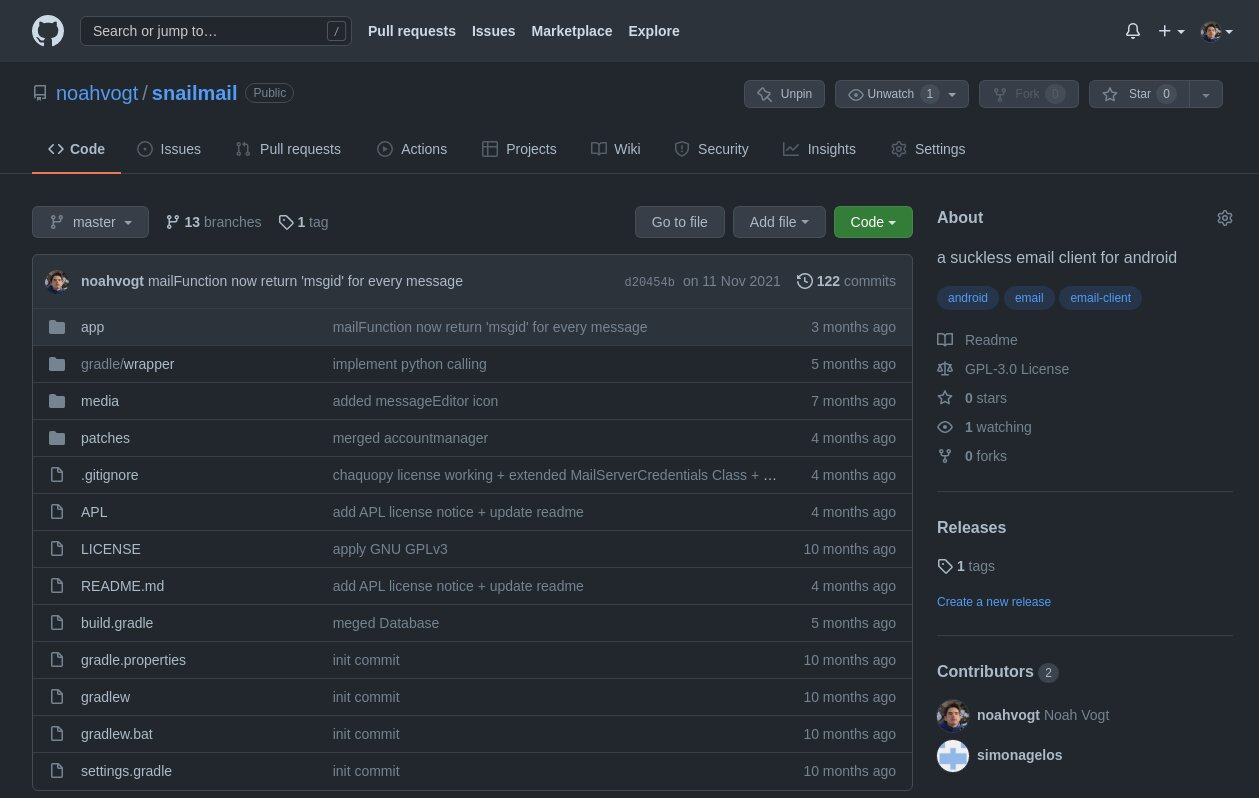
\includegraphics[height=.7\textheight]{media/github-repo.jpg}
    \end{figure}
    \begin{itemize}
        \centering
        \item https://github.com/noahvogt/snailmail
        \item https://git.noahvogt.com/me/snailmail
    \end{itemize}
\end{frame}

\end{document}
